%%%%%%%%%%%%%%
%% Run LaTeX on this file several times to get Table of Contents,
%% cross-references, and citations.

%% If you have font problems, you may edit the w-bookps.sty file
%% to customize the font names to match those on your system.

%% w-bksamp.tex. Current Version: Feb 16, 2012
%%%%%%%%%%%%%%%%%%%%%%%%%%%%%%%%%%%%%%%%%%%%%%%%%%%%%%%%%%%%%%%%
%
%  Sample file for
%  Wiley Book Style, Design No.: SD 001B, 7x10
%  Wiley Book Style, Design No.: SD 004B, 6x9
%
%
%  Prepared by Amy Hendrickson, TeXnology Inc.
%  http://www.texnology.com
%%%%%%%%%%%%%%%%%%%%%%%%%%%%%%%%%%%%%%%%%%%%%%%%%%%%%%%%%%%%%%%%

%%%%%%%%%%%%%
% 7x10
%\documentclass{wileySev}

% 6x9
\documentclass{wileySix}

\usepackage{graphicx}
\usepackage{listings}

\usepackage{color}

\definecolor{codegreen}{rgb}{0,0.6,0}
\definecolor{codegray}{rgb}{0.5,0.5,0.5}
\definecolor{codepurple}{rgb}{0.58,0,0.82}
\definecolor{backcolour}{rgb}{0.95,0.95,0.92}

\lstdefinestyle{mystyle}{
    backgroundcolor=\color{backcolour},
    commentstyle=\color{codegreen},
    keywordstyle=\color{magenta},
    numberstyle=\tiny\color{codegray},
    stringstyle=\color{codepurple},
    basicstyle=\footnotesize,
    breakatwhitespace=false,
    breaklines=true,
    captionpos=b,
    keepspaces=true,
    numbers=left,
    numbersep=5pt,
    showspaces=false,
    showstringspaces=false,
    showtabs=false,
    tabsize=2,
    language=sh
}

\lstset{style=mystyle}

%%%%%%%
%% for times math: However, this package disables bold math (!)
%% \mathbf{x} will still work, but you will not have bold math
%% in section heads or chapter titles. If you don't use math
%% in those environments, mathptmx might be a good choice.

% \usepackage{mathptmx}

% For PostScript text
\usepackage{w-bookps}

%%%%%%%%%%%%%%%%%%%%%%%%%%%%%%%%%%%%%%%%%%%%%%%%%%%%%%%%%%%%%%%%
%% Other packages you might want to use:

% for chapter bibliography made with BibTeX
% \usepackage{chapterbib}

% for multiple indices
% \usepackage{multind}

% for answers to problems
% \usepackage{answers}

%%%%%%%%%%%%%%%%%%%%%%%%%%%%%%
%% Change options here if you want:
%%
%% How many levels of section head would you like numbered?
%% 0= no section numbers, 1= section, 2= subsection, 3= subsubsection
%%==>>
\setcounter{secnumdepth}{3}

%% How many levels of section head would you like to appear in the
%% Table of Contents?
%% 0= chapter titles, 1= section titles, 2= subsection titles,
%% 3= subsubsection titles.
%%==>>
\setcounter{tocdepth}{2}

%% Cropmarks? good for final page makeup
%% \docropmarks

%%%%%%%%%%%%%%%%%%%%%%%%%%%%%%
%
% DRAFT
%
% Uncomment to get double spacing between lines, current date and time
% printed at bottom of page.
% \draft
% (If you want to keep tables from becoming double spaced also uncomment
% this):
% \renewcommand{\arraystretch}{0.6}
%%%%%%%%%%%%%%%%%%%%%%%%%%%%%%

%%%%%%% Demo of section head containing sample macro:
%% To get a macro to expand correctly in a section head, with upper and
%% lower case math, put the definition and set the box
%% before \begin{document}, so that when it appears in the
%% table of contents it will also work:

\newcommand{\VT}[1]{\ensuremath{{V_{T#1}}}}

%% use a box to expand the macro before we put it into the section head:

\newbox\sectsavebox
\setbox\sectsavebox=\hbox{\boldmath\VT{xyz}}

%%%%%%%%%%%%%%%%% End Demo


\begin{document}


\booktitle{Cerdas Menguasai Python}
\subtitle{Dalam 24 Jam}

\authors{Rolly M. Awangga\\
\affil{Informatics Research Center}
%Floyd J. Fowler, Jr.\\
%\affil{University of New Mexico}
}

\offprintinfo{Cerdas Menguasai Python, First Edition}{Rolly M. Awangga}

%% Can use \\ if title, and edition are too wide, ie,
%% \offprintinfo{Survey Methodology,\\ Second Edition}{Robert M. Groves}

%%%%%%%%%%%%%%%%%%%%%%%%%%%%%%
%%
\halftitlepage

%\titlepage


\begin{copyrightpage}{2019}
%Survey Methodology / Robert M. Groves . . . [et al.].
%\       p. cm.---(Wiley series in survey methodology)
%\    ``Wiley-Interscience."
%\    Includes bibliographical references and index.
%\    ISBN 0-471-48348-6 (pbk.)
%\    1. Surveys---Methodology.  2. Social 
%\  sciences---Research---Statistical methods.  I. Groves, Robert M.  II. %
%Series.\\
%
%HA31.2.S873 2007
%001.4'33---dc22                                             2004044064
\end{copyrightpage}

\dedication{`Jika Kamu tidak dapat menahan lelahnya belajar,
Maka kamu harus sanggup menahan perihnya Kebodohan.'
~Imam Syafi'i~}

\begin{contributors}
\name{Rolly Maulana Awangga,} Informatics Research Center., Politeknik Pos Indonesia, Bandung,
Indonesia



\end{contributors}

\contentsinbrief
\tableofcontents
\listoffigures
\listoftables
\lstlistoflistings


\begin{foreword}
Sepatah kata dari Kaprodi, Kabag Kemahasiswaan dan Mahasiswa
\end{foreword}

\begin{preface}
Buku ini diciptakan bagi yang awam dengan flask sekalipun.

\prefaceauthor{R. M. Awangga}
\where{Bandung, Jawa Barat\\
Februari, 2019}
\end{preface}


\begin{acknowledgments}
Terima kasih atas semua masukan dari para mahasiswa agar bisa membuat buku ini 
lebih baik dan lebih mudah dimengerti.

Terima kasih ini juga ditujukan khusus untuk team IRC yang 
telah fokus untuk belajar dan memahami bagaimana buku ini mendampingi proses 
Intership.
\authorinitials{R. M. A.}
\end{acknowledgments}

\begin{acronyms}
\acro{ACGIH}{American Conference of Governmental Industrial Hygienists}
\acro{AEC}{Atomic Energy Commission}
\acro{OSHA}{Occupational Health and Safety Commission}
\acro{SAMA}{Scientific Apparatus Makers Association}
\end{acronyms}

\begin{glossary}
\term{git}Merupakan manajemen sumber kode yang dibuat oleh linus torvald.

\term{bash}Merupakan bahasa sistem operasi berbasiskan *NIX.

\term{linux}Sistem operasi berbasis sumber kode terbuka yang dibuat oleh Linus Torvald
\end{glossary}

\begin{symbols}
\term{A}Amplitude

\term{\hbox{\&}}Propositional logic symbol 

\term{a}Filter Coefficient

\bigskip

\term{\mathcal{B}}Number of Beats
\end{symbols}

\begin{introduction}

%% optional, but if you want to list author:

\introauthor{Rolly Maulana Awangga, S.T., M.T.}
{Informatics Research Center\\
Bandung, Jawa Barat, Indonesia}

Pada era disruptif  \index{disruptif}\index{disruptif!modern} 
saat ini. git merupakan sebuah kebutuhan dalam sebuah organisasi pengembangan perangkat lunak.
Buku ini diharapkan bisa menjadi penghantar para programmer, analis, IT Operation dan Project Manajer.
Dalam melakukan implementasi git pada diri dan organisasinya.

Rumusnya cuman sebagai contoh aja biar keren\cite{awangga2018sampeu}.

\begin{equation}
ABC {\cal DEF} \alpha\beta\Gamma\Delta\sum^{abc}_{def}
\end{equation}

\end{introduction}

%%%%%%%%%%%%%%%%%%Isi Buku_
%TEORI
%\chapter{Judul Bagian Pertama}
%\section{Arjun Yuda Firwanda}
\subsection{Soal 1}
Isi jawaban soal ke-1

Kalau mau dibikin paragrap \textbf{cukup enter aja}, tidak usah pakai \verb|par| dsb

%\subsection{Soal 2}
%Isi jawaban soal ke-2

%\subsection{Soal 3}
%Isi jawaban soal ke-3

\section{Dwi Yulianingsih}
\subsection{Soal 1}
Isi jawaban soal ke-1

Kalau mau dibikin paragrap \textbf{cukup enter aja}, tidak usah pakai \verb|par| dsb

%\subsection{Soal 2}
%Isi jawaban soal ke-2

%\subsection{Soal 3}
%Isi jawaban soal ke-3

\section{Harun Ar-Rasyid}
\subsection{Soal 1}
Isi jawaban soal ke-1

Kalau mau dibikin paragrap \textbf{cukup enter aja}, tidak usah pakai \verb|par| dsb

%\subsection{Soal 2}
%Isi jawaban soal ke-2

%\subsection{Soal 3}
%Isi jawaban soal ke-3

\section{Sri Rahayu}
\subsection{Soal 1}
Isi jawaban soal ke-1

Kalau mau dibikin paragrap \textbf{cukup enter aja}, tidak usah pakai \verb|par| dsb

%\subsection{Soal 2}
%Isi jawaban soal ke-2

%\subsection{Soal 3}
%Isi jawaban soal ke-3

\section{Doli Jonviter}
\subsection{Soal 1}
Isi jawaban soal ke-1

Kalau mau dibikin paragrap \textbf{cukup enter aja}, tidak usah pakai \verb|par| dsb

%\subsection{Soal 2}
%Isi jawaban soal ke-2

%\subsection{Soal 3}
%Isi jawaban soal ke-3

\section{Rahmatul Ridha}
\subsection{Soal 1}
Isi jawaban soal ke-1

Kalau mau dibikin paragrap \textbf{cukup enter aja}, tidak usah pakai \verb|par| dsb

%\subsection{Soal 2}
%Isi jawaban soal ke-2

%\subsection{Soal 3}
%Isi jawaban soal ke-3

\section{Tomy Prawoto}
\subsection{Soal 1}
Isi jawaban soal ke-1

Kalau mau dibikin paragrap \textbf{cukup enter aja}, tidak usah pakai \verb|par| dsb

%\subsection{Soal 2}
%Isi jawaban soal ke-2

%\subsection{Soal 3}
%Isi jawaban soal ke-3

%PRAKTEK
%\chapter{Judul Bagian Pertama}
%\section{Arjun Yuda Firwanda}
\subsection{Soal 1}
Isi jawaban soal ke-1

Kalau mau dibikin paragrap \textbf{cukup enter aja}, tidak usah pakai \verb|par| dsb

%\subsection{Soal 2}
%Isi jawaban soal ke-2

%\subsection{Soal 3}
%Isi jawaban soal ke-3

\section{Dwi Yulianingsih}
\subsection{Soal 1}
Isi jawaban soal ke-1

Kalau mau dibikin paragrap \textbf{cukup enter aja}, tidak usah pakai \verb|par| dsb

%\subsection{Soal 2}
%Isi jawaban soal ke-2

%\subsection{Soal 3}
%Isi jawaban soal ke-3

\section{Harun Ar-Rasyid}
\subsection{Soal 1}
Isi jawaban soal ke-1

Kalau mau dibikin paragrap \textbf{cukup enter aja}, tidak usah pakai \verb|par| dsb

%\subsection{Soal 2}
%Isi jawaban soal ke-2

%\subsection{Soal 3}
%Isi jawaban soal ke-3

\section{Sri Rahayu}
\subsection{Soal 1}
Isi jawaban soal ke-1

Kalau mau dibikin paragrap \textbf{cukup enter aja}, tidak usah pakai \verb|par| dsb

%\subsection{Soal 2}
%Isi jawaban soal ke-2

%\subsection{Soal 3}
%Isi jawaban soal ke-3

\section{Doli Jonviter}
\subsection{Soal 1}
Isi jawaban soal ke-1

Kalau mau dibikin paragrap \textbf{cukup enter aja}, tidak usah pakai \verb|par| dsb

%\subsection{Soal 2}
%Isi jawaban soal ke-2

%\subsection{Soal 3}
%Isi jawaban soal ke-3

\section{Rahmatul Ridha}
\subsection{Soal 1}
Isi jawaban soal ke-1

Kalau mau dibikin paragrap \textbf{cukup enter aja}, tidak usah pakai \verb|par| dsb

%\subsection{Soal 2}
%Isi jawaban soal ke-2

%\subsection{Soal 3}
%Isi jawaban soal ke-3

\section{Tomy Prawoto}
\subsection{Soal 1}
Isi jawaban soal ke-1

Kalau mau dibikin paragrap \textbf{cukup enter aja}, tidak usah pakai \verb|par| dsb

%\subsection{Soal 2}
%Isi jawaban soal ke-2

%\subsection{Soal 3}
%Isi jawaban soal ke-3


%TEORI
%\chapter{Judul Bagian Pertama}
%\section{Arjun Yuda Firwanda}
\subsection{Soal 1}
Isi jawaban soal ke-1

Kalau mau dibikin paragrap \textbf{cukup enter aja}, tidak usah pakai \verb|par| dsb

%\subsection{Soal 2}
%Isi jawaban soal ke-2

%\subsection{Soal 3}
%Isi jawaban soal ke-3

\section{Dwi Yulianingsih}
\subsection{Soal 1}
Isi jawaban soal ke-1

Kalau mau dibikin paragrap \textbf{cukup enter aja}, tidak usah pakai \verb|par| dsb

%\subsection{Soal 2}
%Isi jawaban soal ke-2

%\subsection{Soal 3}
%Isi jawaban soal ke-3

\section{Harun Ar-Rasyid}
\subsection{Soal 1}
Isi jawaban soal ke-1

Kalau mau dibikin paragrap \textbf{cukup enter aja}, tidak usah pakai \verb|par| dsb

%\subsection{Soal 2}
%Isi jawaban soal ke-2

%\subsection{Soal 3}
%Isi jawaban soal ke-3

\section{Sri Rahayu}
\subsection{Soal 1}
Isi jawaban soal ke-1

Kalau mau dibikin paragrap \textbf{cukup enter aja}, tidak usah pakai \verb|par| dsb

%\subsection{Soal 2}
%Isi jawaban soal ke-2

%\subsection{Soal 3}
%Isi jawaban soal ke-3

\section{Doli Jonviter}
\subsection{Soal 1}
Isi jawaban soal ke-1

Kalau mau dibikin paragrap \textbf{cukup enter aja}, tidak usah pakai \verb|par| dsb

%\subsection{Soal 2}
%Isi jawaban soal ke-2

%\subsection{Soal 3}
%Isi jawaban soal ke-3

\section{Rahmatul Ridha}
\subsection{Soal 1}
Isi jawaban soal ke-1

Kalau mau dibikin paragrap \textbf{cukup enter aja}, tidak usah pakai \verb|par| dsb

%\subsection{Soal 2}
%Isi jawaban soal ke-2

%\subsection{Soal 3}
%Isi jawaban soal ke-3

\section{Tomy Prawoto}
\subsection{Soal 1}
Isi jawaban soal ke-1

Kalau mau dibikin paragrap \textbf{cukup enter aja}, tidak usah pakai \verb|par| dsb

%\subsection{Soal 2}
%Isi jawaban soal ke-2

%\subsection{Soal 3}
%Isi jawaban soal ke-3

%PRAKTEK
%\chapter{Judul Bagian Pertama}
%\section{Arjun Yuda Firwanda}
\subsection{Soal 1}
Isi jawaban soal ke-1

Kalau mau dibikin paragrap \textbf{cukup enter aja}, tidak usah pakai \verb|par| dsb

%\subsection{Soal 2}
%Isi jawaban soal ke-2

%\subsection{Soal 3}
%Isi jawaban soal ke-3

\section{Dwi Yulianingsih}
\subsection{Soal 1}
Isi jawaban soal ke-1

Kalau mau dibikin paragrap \textbf{cukup enter aja}, tidak usah pakai \verb|par| dsb

%\subsection{Soal 2}
%Isi jawaban soal ke-2

%\subsection{Soal 3}
%Isi jawaban soal ke-3

\section{Harun Ar-Rasyid}
\subsection{Soal 1}
Isi jawaban soal ke-1

Kalau mau dibikin paragrap \textbf{cukup enter aja}, tidak usah pakai \verb|par| dsb

%\subsection{Soal 2}
%Isi jawaban soal ke-2

%\subsection{Soal 3}
%Isi jawaban soal ke-3

\section{Sri Rahayu}
\subsection{Soal 1}
Isi jawaban soal ke-1

Kalau mau dibikin paragrap \textbf{cukup enter aja}, tidak usah pakai \verb|par| dsb

%\subsection{Soal 2}
%Isi jawaban soal ke-2

%\subsection{Soal 3}
%Isi jawaban soal ke-3

\section{Doli Jonviter}
\subsection{Soal 1}
Isi jawaban soal ke-1

Kalau mau dibikin paragrap \textbf{cukup enter aja}, tidak usah pakai \verb|par| dsb

%\subsection{Soal 2}
%Isi jawaban soal ke-2

%\subsection{Soal 3}
%Isi jawaban soal ke-3

\section{Rahmatul Ridha}
\subsection{Soal 1}
Isi jawaban soal ke-1

Kalau mau dibikin paragrap \textbf{cukup enter aja}, tidak usah pakai \verb|par| dsb

%\subsection{Soal 2}
%Isi jawaban soal ke-2

%\subsection{Soal 3}
%Isi jawaban soal ke-3

\section{Tomy Prawoto}
\subsection{Soal 1}
Isi jawaban soal ke-1

Kalau mau dibikin paragrap \textbf{cukup enter aja}, tidak usah pakai \verb|par| dsb

%\subsection{Soal 2}
%Isi jawaban soal ke-2

%\subsection{Soal 3}
%Isi jawaban soal ke-3


%TEORI
%\chapter{Judul Bagian Pertama}
%\section{Arjun Yuda Firwanda}
\subsection{Soal 1}
Isi jawaban soal ke-1

Kalau mau dibikin paragrap \textbf{cukup enter aja}, tidak usah pakai \verb|par| dsb

%\subsection{Soal 2}
%Isi jawaban soal ke-2

%\subsection{Soal 3}
%Isi jawaban soal ke-3

\section{Dwi Yulianingsih}
\subsection{Soal 1}
Isi jawaban soal ke-1

Kalau mau dibikin paragrap \textbf{cukup enter aja}, tidak usah pakai \verb|par| dsb

%\subsection{Soal 2}
%Isi jawaban soal ke-2

%\subsection{Soal 3}
%Isi jawaban soal ke-3

\section{Harun Ar-Rasyid}
\subsection{Soal 1}
Isi jawaban soal ke-1

Kalau mau dibikin paragrap \textbf{cukup enter aja}, tidak usah pakai \verb|par| dsb

%\subsection{Soal 2}
%Isi jawaban soal ke-2

%\subsection{Soal 3}
%Isi jawaban soal ke-3

\section{Sri Rahayu}
\subsection{Soal 1}
Isi jawaban soal ke-1

Kalau mau dibikin paragrap \textbf{cukup enter aja}, tidak usah pakai \verb|par| dsb

%\subsection{Soal 2}
%Isi jawaban soal ke-2

%\subsection{Soal 3}
%Isi jawaban soal ke-3

\section{Doli Jonviter}
\subsection{Soal 1}
Isi jawaban soal ke-1

Kalau mau dibikin paragrap \textbf{cukup enter aja}, tidak usah pakai \verb|par| dsb

%\subsection{Soal 2}
%Isi jawaban soal ke-2

%\subsection{Soal 3}
%Isi jawaban soal ke-3

\section{Rahmatul Ridha}
\subsection{Soal 1}
Isi jawaban soal ke-1

Kalau mau dibikin paragrap \textbf{cukup enter aja}, tidak usah pakai \verb|par| dsb

%\subsection{Soal 2}
%Isi jawaban soal ke-2

%\subsection{Soal 3}
%Isi jawaban soal ke-3

\section{Tomy Prawoto}
\subsection{Soal 1}
Isi jawaban soal ke-1

Kalau mau dibikin paragrap \textbf{cukup enter aja}, tidak usah pakai \verb|par| dsb

%\subsection{Soal 2}
%Isi jawaban soal ke-2

%\subsection{Soal 3}
%Isi jawaban soal ke-3

%PRAKTEK
%\chapter{Judul Bagian Pertama}
%\section{Arjun Yuda Firwanda}
\subsection{Soal 1}
Isi jawaban soal ke-1

Kalau mau dibikin paragrap \textbf{cukup enter aja}, tidak usah pakai \verb|par| dsb

%\subsection{Soal 2}
%Isi jawaban soal ke-2

%\subsection{Soal 3}
%Isi jawaban soal ke-3

\section{Dwi Yulianingsih}
\subsection{Soal 1}
Isi jawaban soal ke-1

Kalau mau dibikin paragrap \textbf{cukup enter aja}, tidak usah pakai \verb|par| dsb

%\subsection{Soal 2}
%Isi jawaban soal ke-2

%\subsection{Soal 3}
%Isi jawaban soal ke-3

\section{Harun Ar-Rasyid}
\subsection{Soal 1}
Isi jawaban soal ke-1

Kalau mau dibikin paragrap \textbf{cukup enter aja}, tidak usah pakai \verb|par| dsb

%\subsection{Soal 2}
%Isi jawaban soal ke-2

%\subsection{Soal 3}
%Isi jawaban soal ke-3

\section{Sri Rahayu}
\subsection{Soal 1}
Isi jawaban soal ke-1

Kalau mau dibikin paragrap \textbf{cukup enter aja}, tidak usah pakai \verb|par| dsb

%\subsection{Soal 2}
%Isi jawaban soal ke-2

%\subsection{Soal 3}
%Isi jawaban soal ke-3

\section{Doli Jonviter}
\subsection{Soal 1}
Isi jawaban soal ke-1

Kalau mau dibikin paragrap \textbf{cukup enter aja}, tidak usah pakai \verb|par| dsb

%\subsection{Soal 2}
%Isi jawaban soal ke-2

%\subsection{Soal 3}
%Isi jawaban soal ke-3

\section{Rahmatul Ridha}
\subsection{Soal 1}
Isi jawaban soal ke-1

Kalau mau dibikin paragrap \textbf{cukup enter aja}, tidak usah pakai \verb|par| dsb

%\subsection{Soal 2}
%Isi jawaban soal ke-2

%\subsection{Soal 3}
%Isi jawaban soal ke-3

\section{Tomy Prawoto}
\subsection{Soal 1}
Isi jawaban soal ke-1

Kalau mau dibikin paragrap \textbf{cukup enter aja}, tidak usah pakai \verb|par| dsb

%\subsection{Soal 2}
%Isi jawaban soal ke-2

%\subsection{Soal 3}
%Isi jawaban soal ke-3


%TEORI
\chapter{Library CSV dan Pandas}
\section{Luthfi Muhammad Nabil/1174035}
\subsection{Soal 1}
Fungsi, Sejarah, dan Contoh file CSV : 
\begin{itemize}
	\item Fungsi : 
	File CSV (Comma Separated Values) adalah tipe file khusus yang menyimpan informasi dengan metode dipisahkan dengan koma. File CSV berfungsi untuk menjadi perantara untuk beberapa aplikasi yang memiliki basis data saat mengirim data. CSV dapat dibuka di berbagai text editor
	yang ada. Dengan bentuk filenya yang dinamis memungkinkan file CSV dapat dimanipulasi dan dapat menyimpan informasi dengan skala besar.
	\item Sejarah :
	CSV sudah digunakan sejak tahun 1972 yang dapat dikompilasi pada bahasa pemrograman IBM Fortran. Saat itu, data yang dipisahkan oleh koma jika isinya memiliki spasi maka harus diberi tanda petik di awal dan akhir isi dari data tersebut. Nama CSV baru mulai digunakan pada tahun 1983. Pada panduan dari Osborne Executive Computer mendokumentasikan kutipan yang membolehkan isi karakter memiliki koma.  Pada tahun 2005 dengan RFC4180, CSV didefinisikan sebagai MIME Content Type. lalu pada tahun 2013, defisiensi dari RFC4180 dipecahkan oleh rekomendasi dari W3C. Pada tahun 2014, IETF mempublikasi RFC7111 yang mendeskripsikan pecahan Uniform Resource Identifier(URI) ke dokumen CSV. RFC7111 menjelaskan bagaimana baris, kolom dapat dipilih dalam dokumen CSV menggunakan indeks posisi. Pada Tahun 2015, W3C mempublikasikan draft rekomendasi untuk CSV-metadata standards yang dimulai dengan rekomendasi pada bulan Desember dengan tahun yang sama. 
	\item Contoh File CSV \begin{itemize}
							\item 
							CSV pada Excel \ref{1174035_CSVExcel}
							\begin{figure}[!htbp]
								\centering
								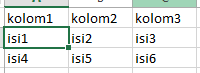
\includegraphics[height=4cm, width=7cm]{figures/4/1174035/Teori/1174035_CSVExcel.jpg}
								\caption{Contoh CSV Pada Excel}
								\label{1174035_CSVExcel}
							\end{figure}
							\item \begin{figure}[!htbp]
								\centering
								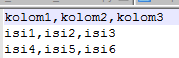
\includegraphics[height=4cm, width=7cm]{figures/4/1174035/Teori/1174035_CSVText.jpg}
								\caption{Contoh CSV Pada Text}
								\label{1174035_CSVText}
							\end{figure}
							CSV pada Text Editor \ref{1174035_CSVText}
							
						  \end{itemize}
\end{itemize}
\subsection{Soal 2}
Aplikasi Yang dapat membuat file CSV : 
Berikut file yang dapat membuat file CSV
\begin{itemize}
	\item Spreadsheet :
	Spreadsheet merupakan aplikasi yang dapat membuat CSV hanya dengan memasukan data sesuai baris dan kolom yang diinginkan. Contoh spreadsheet seperti Google Spreadsheet, Microsoft Excel, dan aplikasi lainnya. 
	\item Bahasa Pemrograman :
	Bahasa pemrograman merupakan media yang dapat untuk membuat aplikasi yang dapat membuat file CSV khusus untuk bahasa pemrograman yang support dengan pembuatan file CSV. Seperti Python, C Sharp, dan lain sebagainya.
	\item Text Editor :
	Text editor juga dapat membuat file CSV, untuk membuat dengan Text Editor cukup dengan membuat file sesuai format CSV dan save file tersebut dengan ekstensi .CSV.
\end{itemize}
\subsection{Soal 3}
Menulis dan Membaca file CSV : 
Berikut cara menulis dan membaca file CSV : 
\begin{itemize}
	\item Menulis : \begin{enumerate}
						\item Buka file CSV dengan spreadsheet
						\item Klik Cell yang mau diisi
						\item Masukan data yang mau diisi pada cell tersebut
						\item Lalu save file dengan format .CSV
					\end{enumerate}
	\item Membaca : \begin{enumerate}
						\item Buka file CSV dengan spreadsheet						
					\end{enumerate}
\end{itemize}
\subsection{Soal 4}
Sejarah Library CSV Python : 
Library CSV pada python merupakan library yang paling umum untuk import export data pada spreadsheet dan basis data dengan format sesuai dengan standarisasi RFC4180. Seiring dengan lahirnya bahasa pemrograman python, library mulai dibuat dan dikembangkan sampai akhirnya pada tahun 2003, pembuatnya Kevin Altis dan lainnya telah merilis versi final untuk library Python CSV. 
\subsection{Soal 5}
Sejarah Library Pandas Python : 
Pandas (Python Data Analysis Library) adalah library open source yang digunakan untuk melakukan data manajemen dan data analysis. Pandas diciptakan pada tahun 2008 oleh Wes McKinney dan diperbaharui oleh Sien Chang pada tahun 2010. Inspirasi dari pembuatan pandas muncul pada komunitas yang membutuhkan library khusus untuk analisis data. 
\subsection{Soal 6}
Fungsi - fungsi yang terdapat di library CSV : 
\begin{itemize}
	\item \begin{verbatim} csv.reader(csvfile, dialect='excel', **fmtparams) \end{verbatim} Untuk mengembalikan	object reader yang akan mengambil setiap line pada csv yang diambil. Data setiap baris diambil saat next() dipanggil. Berikut contohnya : \lstinputlisting[firstline=1, lastline=6]{src/4/1174035/Teori/chap4_1174035_teori.py}
	\item \begin{verbatim} csv.writer(csvfile, dialect='excel', **fmtparams) \end{verbatim} Mengembalikan file pembuat object untuk dapat mengkonversi data pada python ke file CSV yang akan dibuat. Berikut contoh penggunaan csv.writer : \lstinputlisting[firstline=8, lastline=14]{src/4/1174035/Teori/chap4_1174035_teori.py}
	\item \begin{verbatim} csv.register_dialect(name[, dialect[, **fmtparams]]) \end{verbatim} Mengasosiasikan dialek dengan nama, nama yang dimasukkan harus berupa karakter.
	\item \begin{verbatim} csv.unregister_dialect(name) \end{verbatim}
	Menghapus asosiasi dialek dengan nama pada registry dialek.
	\item \begin{verbatim} csv.get_dialect(name) \end{verbatim}
	Mengambil dialek yang telah diasosiasikan dengan nama. 
	\item \begin{verbatim}  csv.list_dialects() \end{verbatim} Mengembalikan dialek yang telah diregistrasi.
	\item \begin{verbatim} csv.field_size_limit([new_limit]) \end{verbatim} Mengembalikan maksimal kolom data yang diperbolehkan oleh pembaca.
\end{itemize}
\subsection{Soal 7}
Fungsi - fungsi yang terdapat di library Pandas : 
\begin{itemize}
	\item \begin{verbatim} pandas.read_csv(filepath_or_buffer[, sep, …]) \end{verbatim} Untuk membaca file CSV dan menyimpannya ke DataFrame
	\item \begin{verbatim} pandas.read_excel(io[, sheet_name, header, names, …])  \end{verbatim} Membaca file excel dan menyimpannya ke DataFrame
	\item \begin{verbatim} to_csv([path, index, sep, na_rep, …]) \end{verbatim}
	Untuk membuat file CSV dari data yang ada	
\end{itemize}
\subsection{Cek Plagiarism}
Berikut pengecekan plagiarism yang dilakukan pada website smallseotools.com : 
\begin{figure}[!htbp]
	\centering
	\includegraphics[height=6cm, width=10cm]{figures/4/1174035/Teori/1174035_plagiarism.png}
	\caption{Cek Plagiarisme}
	\label{1174035_plagiarism}
\end{figure}

\section{Hagan Rowlenstino/1174040}
	\subsection{Soal 1}
	format file csv dapat menyimpan data dalam jumlah yang sangat besar juga diperuntukkan untuk export dan import untuk spreadsheet ataupun database. Singkatan CSV pertamakali di pakai pada tahun 1983, dimana value yang dipisahkan dengan koma lebih mudah untuk diketik daripada data yang sejajar dengan kolom yang tetap. contohnya seperti gambar dibawah ini.

	\begin{figure}[ht]
            \centerline{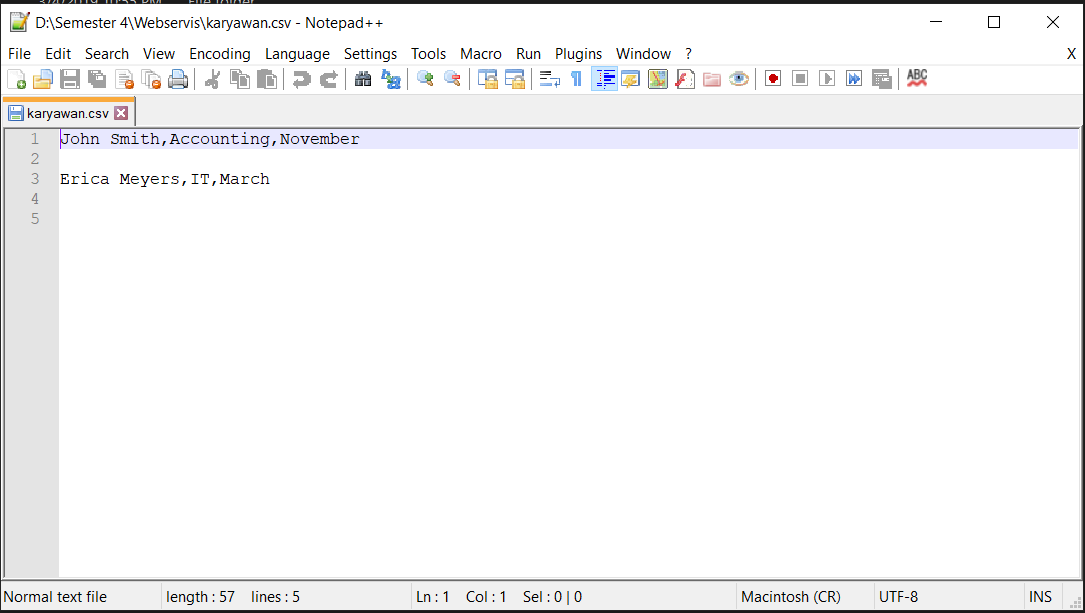
\includegraphics[width=0.5\textwidth]{figures/4/1174040/Teori/1174040_csv.png}}
            \caption{Contoh CSV}
            \label{1174040_csv}
            \end{figure}

    \subsection{Soal 2}
    Ms.Excel , NotePad, notepad++, sublime, dan texteditor lainnya

    \subsection{Soal 3}
    caranya adalah :
		\begin{itemize}
			\item untuk write :
			\begin{enumerate}
				\item Download template csv
				\item Buka browser lalu menuju ke Google Sheet
				\item Tekan tombol merah di pojok kanan bawah
				\item Lalu pilih upload file untuk mengupload template yang sudah di download sebelumya
				\item Edit sesuai yang diinginkan
				\item Setelah selesai, lalukan eksport ke CSV dengan cara klik file lalu download as setelah itu pilih CSV
			\end{enumerate}
			\item untuk read :
			\begin{enumerate}
				\item buka Ms.Excel
				\item pilih Data lalu Get External Data dan pilih From Text
				\item lalu pilih file csv nya
				\item pilih Delimeted lalu Next
				\item checklist di box Tab dan Comma
				\item lalu klik finish
			\end{enumerate}
		\end{itemize}

	\subsection{Soal 4}
	Library umum dalam CSV yang gunanya untuk import dan export data di dalam database yang terstandarisasi RFC4180 yang berisikan fungsi -fungsi dan kelas yang akan dipakai dalam pengerjaan file CSV.

	\subsection{Soal 5}
	Pandas diciptakan pada tahun 2008 oleh Wes McKinney dan diperbaharuin pada tahun 2010 oleh Sien Chang. yang fungsinya untuk melakukan analisa data seperti import dan export data.

	\subsection{Soal 6}
	Fungsi - funsi library csv adalah :
		\begin{itemize}
			
			\item \begin{verbatim}csv.reader(csvfile, dialect='excel', **fmtparams)\end{verbatim} : digunakan untuk membaca line di csv
			\item \begin{verbatim}csv.writer(csvfile, dialect='excel', **fmtparams)\end{verbatim} : untuk menulis line di csv
			\item \begin{verbatim}csv.register_dialect(name[, dialect[, **fmtparams]]) \end{verbatim}: untuk asosiasikan dialect dengan name, dimana name harus string
			\item \begin{verbatim}csv.unregister_dialect(name)\end{verbatim} : menghapus dialect yang terasosiasi dengan name
			\item \begin{verbatim}csv.get_dialect(name)\end{verbatim} : mengnembalikan hasil dialect yang terasosisasi dengan name
			\item \begin{verbatim}csv.list_dialects() \end{verbatim}: menampilkan semua dialect yang ada
			\item \begin{verbatim}csv.field_size_limit([new_limit])\end{verbatim} : menamplikan field maksimal ayng di berikan oleh pembubat parse.

		\end{itemize}

	\subsection{Soal 7}
	Fungsi - fungsi yang terdapat di library Pandas : 
\begin{itemize}
	\item \begin{verbatim} pandas.read_csv(filepath_or_buffer[, sep, …]) \end{verbatim} : Untuk membaca file CSV
	\item \begin{verbatim} pandas.read_excel(io[, sheet_name, header, names, …])  \end{verbatim} : Membaca file excel 
	\item \begin{verbatim} to_csv([path, index, sep, na_rep, …]) \end{verbatim} : Untuk me write ke dalam file csv	
\end{itemize}
	
	\subsection{Cek Plagiarisme}
	\begin{figure}[ht]
            \centerline{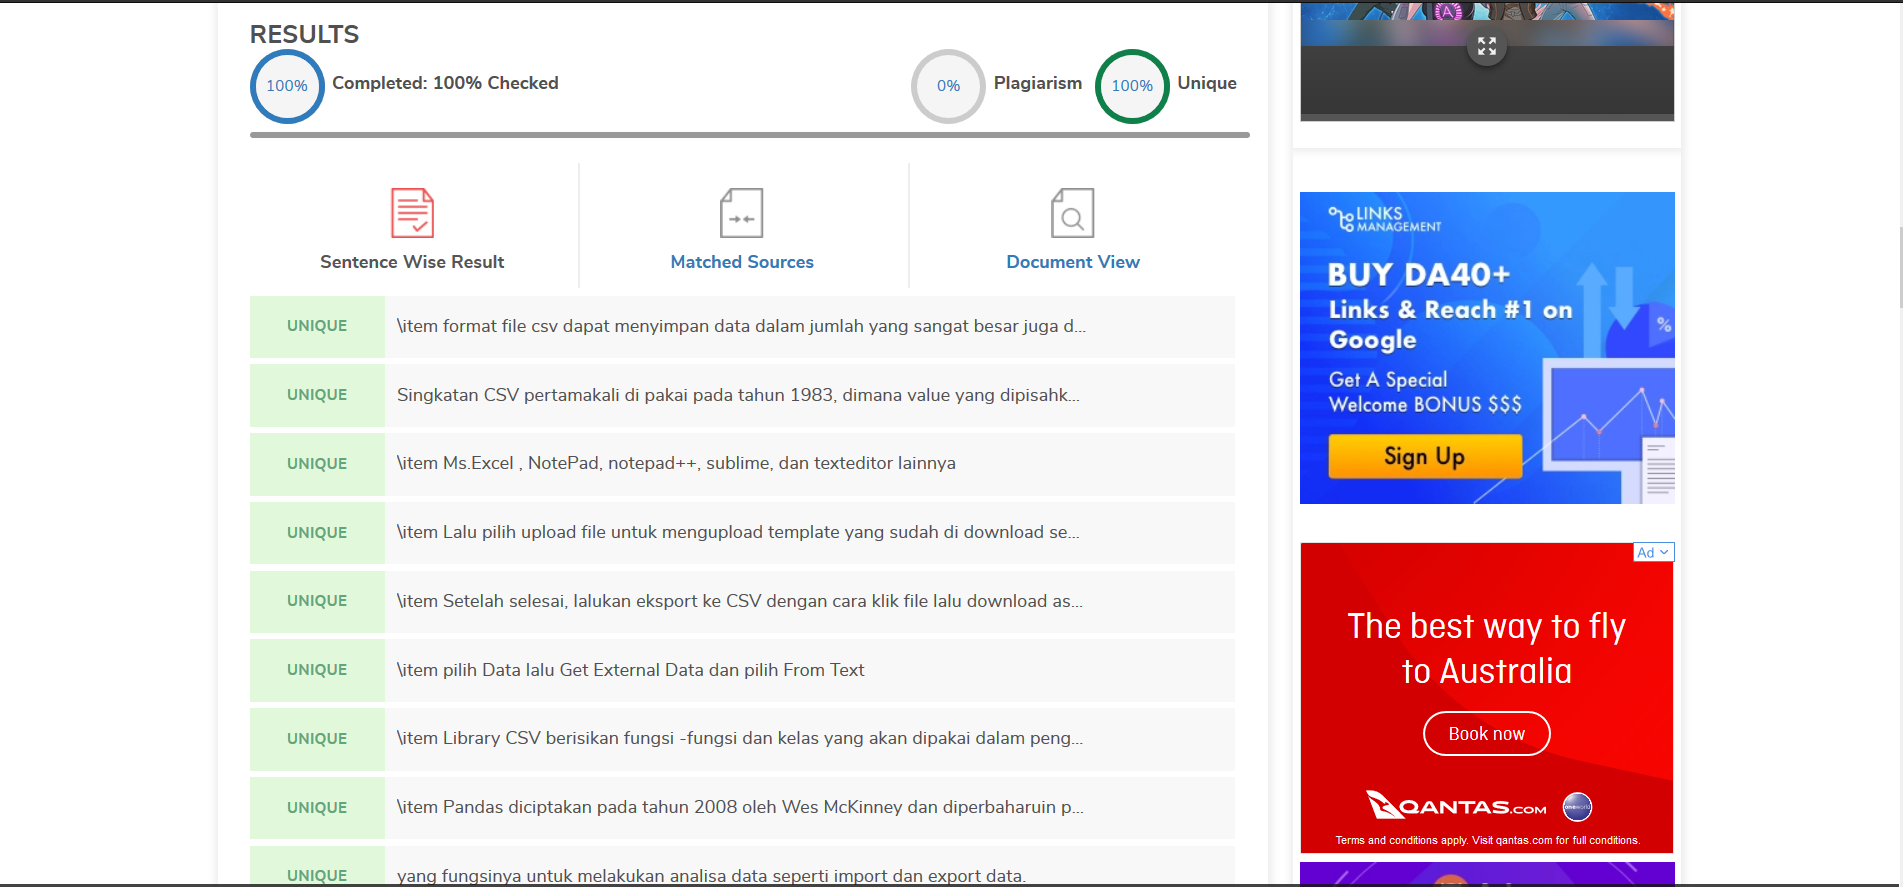
\includegraphics[width=0.5\textwidth]{figures/4/1174040/Teori/1174040_plagiat.png}}
            \caption{Plagiarisme}
            \label{1174040_plagiat}
            \end{figure}
			

\section{Faisal Najib Abdullah 1174042}
\subsection{Pemahaman Teori}
\begin{enumerate}
    \item Apa itu fungsi file csv, jelaskan sejarah dan contoh ?
    \par
    File CSV Nilai Berbatas Koma adalah tipe file khusus yang dapat Anda buat atau edit di Excel. File CSV menyimpan informasi yang dipisahkan oleh koma, bukan menyimpan informasi dalam kolom. Saat teks dan angka disimpan dalam file CSV, mudah untuk memindahkannya dari satu program ke program lain.
    \par 
	File CSV dibuat oleh program yang menangani sejumlah data yang besar. CSV merupakan cara yang nyaman untuk mengekspor data dari spreadsheet dan basis data serta mengimpor atau menggunakannya dalam program lain. Misalnya, Anda dapat mengekspor hasil program penambangan data ke file CSV dan kemudian mengimpornya ke dalam spreadsheet untuk menganalisis data, menghasilkan grafik untuk presentasi, atau menyiapkan laporan untuk publikasi.
    \par
	Contohnya, Anda dapat mengekspor kontak dari Google ke dalam file CSV, kemudian mengimpornya ke Outlook.
    
    \item Aplikasi-aplikasi apa saja yang bisa menciptakan file csv?
    Pada Windows
    \begin{itemize}
        \item Microsoft Excel 2013
        \item Microsoft Works
        \item CCorel Quattro Pro
        \item Apache OpenOffice
        \item LibreOffice
        \item Microsoft Notepad
        \item Intuit Quicken 2015
        \item GenScriber
    \end{itemize}
    Pada Mac OS
    \begin{itemize}
        \item Microsoft Excel 2011
        \item Planamesa NeoOffice
        \item Apache OpenOffice
        \item LibreOffice
        \item GenScriber
    \end{itemize}
    Pada Linux
    \begin{itemize}
        \item Apache OpenOffice
        \item LibreOffice
        \item GenScriber
    \end{itemize}
    
    \item Jelaskan bagaimana cara menulis dan membaca file csv di excel atau spreadsheet?
	\begin{itemize}
        \item Cara menulis file csv harus berupa baris dan kolom atau bisa juga di sebut berupa tabel.
        \item Untuk membacanya file csv dipisahkannya menggunakan koma atau titik koma.
    \end{itemize}
    
    \item Jelaskan sejarah library csv?
	Library csv menyediakan fungsionalitas untuk membaca dan menulis ke file CSV. Dirancang untuk bekerja di luar kotak dengan file CSV yang dihasilkan Excel, memudahkan untuk bekerja dengan berbagai format CSV. Library csv berisi objek dan kode lain untuk membaca, menulis, dan memproses data ke file CSV.
    
    \item Jelaskan sejarah library pandas?
	panda adalah pustaka Python open-source yang menyediakan alat analisis data kinerja tinggi dan struktur data yang mudah digunakan. panda tersedia untuk semua instalasi Python, tetapi itu adalah bagian penting dari distribusi Anaconda dan bekerja sangat baik di notebook Jupyter untuk berbagi data, kode, hasil analisis, visualisasi, dan teks naratif.

    \item Jelaskan fungsi-fungsi yang terdapat di library csv?
	Terdapat 2 fungsi yang bisa digunakan oleh library csv
    Pertama,fungsi membaca file csv.
    fungsi ini bisa menggunakan list dan dictionary
    Dengan list :
    \lstinputlisting[firstline=11, lastline=21]{src/4/1174042/Teori/1174042_csv.py}
    Dengan dictionary :
    \lstinputlisting[firstline=24, lastline=33]{src/4/1174042/Teori/1174042_csv.py}
    Kedua,fungsi menulis file csv.
    \lstinputlisting[firstline=36, lastline=40]{src/4/1174042/Teori/1174042_csv.py}
    
    \item Jelaskan fungsi-fungsi yang terdapat di library pandas
	Hampir sama dengan library csv,tp library pandas penulisannya lebih sederhana dan terlihat lebih rapih dari pada library csv.
    \lstinputlisting[firstline=43, lastline=44]{src/4/1174042/Teori/1174042_csv.py}
\end{enumerate}

\subsection{Cek Plagiarism}
Berikut pengecekan plagiarism yang dilakukan pada website smallseotools.com : 
\begin{figure}[!htbp]
	\centering
	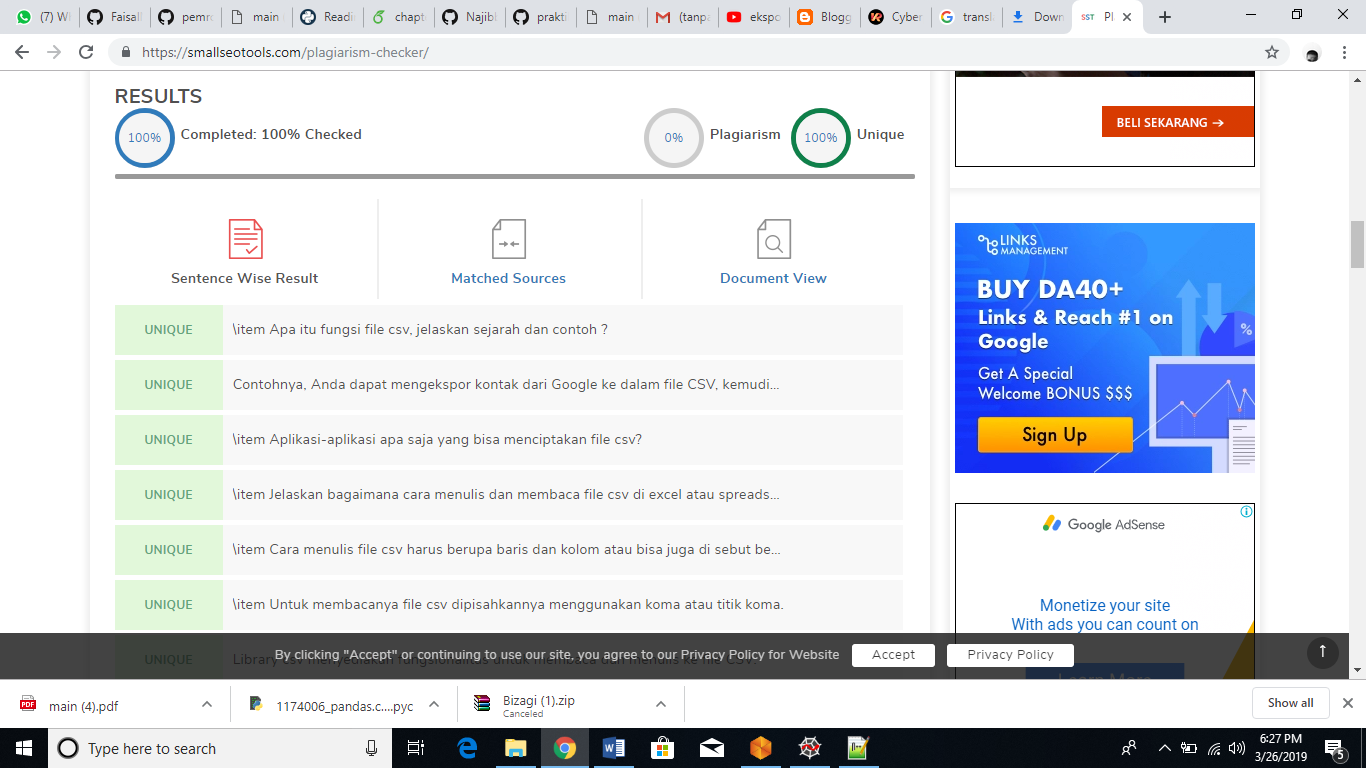
\includegraphics[height=6cm, width=10cm]{figures/4/1174042/1174042_plagiat.png}
	\caption{Cek Plagiarisme}
	\label{}
\end{figure}
%PRAKTEK
\chapter{Praktek Library CSV dan Pandas}
\section{Luthfi Muhammad Nabil/1174035}
\subsection{Soal 1}
Buatlah fungsi pada file chap4\_1174035\_csv.py untuk membuka file csv dengan lib csv mode list : 
\lstinputlisting[firstline=2, lastline=6]{src/4/1174035/Praktek/chap4_1174035_csv.py}

\subsection{Soal 2}
Buatlah fungsi pada file chap4\_1174035\_csv.py untuk membuka file csv dengan lib csv mode dictionary : 
\lstinputlisting[firstline=8, lastline=12]{src/4/1174035/Praktek/chap4_1174035_csv.py}

\subsection{Soal 3}
Buatlah fungsi pada file chap4\_1174035\_pandas.py untuk membuka file csv dengan lib pandas mode list : 
\lstinputlisting[firstline=2, lastline=5]{src/4/1174035/Praktek/chap4_1174035_pandas.py}

\subsection{Soal 4}
Buatlah fungsi pada file chap4\_1174035\_pandas.py untuk membuka file csv dengan lib pandas mode dictionary : 
\lstinputlisting[firstline=6, lastline=10]{src/4/1174035/Praktek/chap4_1174035_pandas.py}

\subsection{Soal 5}
Buatlah fungsi baru di chap4\_1174035\_pandas.py untuk mengubah format tanggal menjadi standard dataframe : 
\lstinputlisting[firstline=11, lastline=13]{src/4/1174035/Praktek/chap4_1174035_pandas.py}

\subsection{Soal 6}
Buatlah fungsi baru di chap4\_1174035\_pandas.py untuk mengubah index kolom : 
\lstinputlisting[firstline=14, lastline=16]{src/4/1174035/Praktek/chap4_1174035_pandas.py}

\subsection{Soal 7}
Buatlah fungsi baru di chap4\_1174035\_pandas.py untuk mengubah atribut atau nama kolom : 
\lstinputlisting[firstline=17, lastline=19]{src/4/1174035/Praktek/chap4_1174035_pandas.py}

\subsection{Soal 8}
Buatlah program chap4\_1174035\_main.py yang menggunakan library chap4\_1174035\_csv.py yang membuat dan membaca file CSV : 
\lstinputlisting{src/4/1174035/Praktek/chap4_1174035_main.py}

\subsection{Soal 9}
Buatlah program chap4\_1174035\_main2.py yang menggunakan library chap4\_1174035\_csv.py yang membuat dan membaca file CSV : 
\lstinputlisting{src/4/1174035/Praktek/chap4_1174035_main2.py}

\subsection{Penanganan Error}
Error yang didapat : KeyError
Deskripsi : Error saat kunci ada yang salah atau tidak ada di dalam file CSV 
\begin{figure}[!htbp]
	\centering
	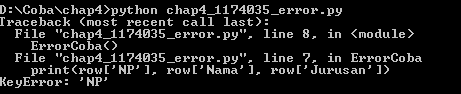
\includegraphics[height=4cm, width=10cm]{figures/4/1174035/Praktek/chap4_1174035_error.png}
	\caption{Contoh KeyError}
	\label{1174035_Error}
\end{figure}
Penanganan : Menggunakan KeyError seperti pada line berikut : \lstinputlisting{src/4/1174035/Praktek/chap4_1174035_error.py}
\begin{figure}[!htbp]
	\centering
	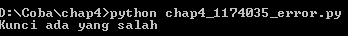
\includegraphics[height=4cm, width=10cm]{figures/4/1174035/Praktek/chap4_1174035_errorfix.png}
	\caption{Hasil Penanganan Error}
	\label{1174035_ErrorFix}
\end{figure}

\section{Hagan Rowlenstino/1174040}
\subsection{Soal 1}
Buatlah fungsi untuk membuka file csv dengan lib csv mode list : 
\lstinputlisting{src/4/1174040/Praktek/1174040_CSV1.py}

\subsection{Soal 2}
Buatlah fungsi untuk membuka file csv dengan lib csv mode dictionary : 
\lstinputlisting{src/4/1174040/Praktek/1174040_CSV2.py}

\subsection{Soal 3}
Buatlah fungsi  untuk membuka file csv dengan lib pandas mode list : 
\lstinputlisting{src/4/1174040/Praktek/1174040_pandas1.py}

\subsection{Soal 4}
Buatlah fungsi  untuk membuka file csv dengan lib pandas mode dictionary : 
\lstinputlisting{src/4/1174040/Praktek/1174040_pandas2.py}

\subsection{Soal 5}
Buatlah fungsi untuk mengubah format tanggal menjadi standard dataframe : 
\lstinputlisting{src/4/1174040/Praktek/1174040_pandas3.py}

\subsection{Soal 6}
Buatlah fungsi  untuk mengubah index kolom : 
\lstinputlisting{src/4/1174040/Praktek/1174040_pandas4.py}

\subsection{Soal 7}
Buatlah fungsi  untuk mengubah atribut atau nama kolom : 
\lstinputlisting{src/4/1174040/Praktek/1174040_pandas5.py}

\subsection{Soal 8}
Disini saya telah membuat file CSV bernama 1174040\_csv.csv untuk di tampilkan, dan sebelum me write ke dalam file csv, terlebih dahulu buat file 1174040\_writecsv.csv : 
\lstinputlisting{src/4/1174040/Praktek/1174040_main.py}

\subsection{Soal 9}
Disini saya telah membuat file CSV bernama 1174040\_csvpandas.csv untuk ditampilkan, dan sebelum me write ke dalam file csv, telebih dahulu buat file 1174040\_writepandas.csv : 
\lstinputlisting{src/4/1174040/Praktek/1174040_main2.py}

\chapter{Library CSV dan Pandas}
\section{Irvan Rizkiansyah/1174043}
	\subsection{Soal 1}
		\begin{itemize}
			\item Device Manager pada windows berfungsi untuk menampilkan segala macam perangkat hardware yang ter-inisialisasi oleh windows itu sendiri, dan juga berguna dalam mengelola perangkat hardware yang terpasang dan terdeteksi oleh windows.
			
			\item Direktori /dev pada linux pun berguna seperti device manager pada windows, dimana pada direktori /dev ini tersimpan konfigurasi perangkat device ataupun hardware yang terdeteksi oleh sistem.
			
		\end{itemize}
	\subsection{Soal 2}
	Langkah - langkah instalasi driver arduino :
		\begin{enumerate}
			\item Download terlebih dahulu driver arduino yang di sediakan di website arduino
			\item Kemudian hubungkan arduino ke PC, dan PC akan mendeteksi adanya perangkat yang terhubung namun tidak terbaca perangkat tersebut perangkat apa.
			\item Kemudian buka Device Manager
			\item Lalu pilih dan klik kanan pada perangkat arduino yg terdeteksi
			\item Kemudian pilih install driver atau update driver
			\item Nanti akan muncul pilihan mencari driver secara online atau mencari driver offline, pilih yang offline
			\item Cari file installer driver arduino yang sudah di download sebelumnya, kemudian pilih file installer driver arduino tersebut. dan akan langsung memulai peng-instal-an
			\item Tunggu hingga selesai dan pencet OK, maka driver arduino sudah ter-install
			
		\end{enumerate}
	\subsection{Soal 3}
	Di perlukan melakukan instalasi aplikasi arduino IDE untuk melihat dan mengecek baud rate dan port arduino kita yang terpasang, dengan memilih menu Tools kemudian pilih Serial monitor untuk melihat baud rate dan port dimana arduino yang terpasang.
	
	\subsection{Soal 4}
	Pada tahun 2002 PySerial pertama kalinya di luncurkan, dimana PySerial ini digunakan untuk berkomunikasi dengan mikrokontroller. Kemudian Library PySerial dikembangkan hingga sekarang.
	
	\subsection{Soal 5}
	Fungsi - fungsi yang ada pada PySerial :
		\begin{itemize}
			\item \begin{verbatim}open()\end{verbatim} 
			Berfungsi untuk membuka dan memberikan akses port serial yang terhubung
			\item \begin{verbatim}close()\end{verbatim} 
			Berfungsi untuk memberhentikan akses port serial yang terhubung
			\item \begin{verbatim}flush() \end{verbatim}
			Berfungsi untuk menghapus seluruh data yang ditampilkan, dan masih banyak yang lainnya.
			
		\end{itemize}
	
	\subsection{Soal 6}
	Dengan perulangan kita dapat melihat perkembangan dari mikrokontroller yang sedangn berjalan dari awal hingga akhir, apakah ada hal yang aneh, dengan perulangan semua data terbaca.
	Akan tetapi ada saat dimana perulangan tidak dibutuhkan, misalnya seperti kita hanya membutuhkan data hasil mikrokontroller yang berjalan pada saat tertentu saja, maka tanpa perulangan pun berguna.
	
	\subsection{Soal 7}
	Dalam membuat fungsi pada PySerial kita hanya perlua menginisialisasikan pembuatan fungsi seperti pada biasanya seperti : \begin{verbatim} def nama_fungsi() \end{verbatim}


\section{Hagan Rowlenstino/1174040}
	\subsection{Soal 1} 
		\begin{itemize}
			\item Device Manager : Seperti namanya sendiri, device manager berfungsi untuk menampilkan dan mengelola semua hardware yang terinstall ataupun dapat di instalasi ke dalam windows.

			\item folder /dev : Di dalam sistem operasi Linux, perangkat yang tehubung akan dianggap sebagai file. di dalam folder /dev inilah file - file  tersebut berada.
		\end{itemize}

	\subsection{Soal 2}
	Langkah - langkah instalasi driver arduino :
		\begin{enumerate}
			\item download file driver arduino terlebih dahulu dan masukkan ke dalam directory yang diinginkan
			\item hubungkan arduinio uno anda ke pc anda dengan kabel USB yang tersedia
			\item lalu windows akan memunculkan pop up yang memberitahu bahwa ingin menginstall dirver, tapi nanti tidak akan menemukan drivernya
			\item buka Device Manager 
			\item cari unknown device di dalam Device Manager di dalam tab other device
			\item klik kanan pada unknown device tersebut lalu pilih update driver software
			\item pilih browse my computer for driver software lalu masukkan directory dimana anda menyimpan driver arduino yang telah anda download tadi
			\item setelah itu klik install dan tunggu hingga proses selesai
			\item arduino pun sudah terbaca di pc anda 
		\end{enumerate}

	\subsection{Soal 3}
	Untuk melihat atau membaca baudrate dan port kita hanya perlu menginstall Arduino IDE, setelah itu buka menu serial monitor yang berada di tab tools. Dari sana akan terlihat baik baudrate dan port yang sedang digunakan oleh arduin anda.

	\subsection{Soal 4}
	PySerial merupakan sebuah library yang digunakan untuk komunikasi ke port serial terutama untuk mikrokontroller. PySerial pertama kali diluncurkan pada tahun 2002 yang makin berkembang dalam setiap versinya hingga tahun 2017 lalu.

	\subsection{Soal 5}
		\begin{itemize}
			\item \begin{verbatim}stop()\end{verbatim} : untuk menghentikan pembacaan program
			\item \begin{verbatim}serial.to_bytes(sequence)\end{verbatim} : berfungsi untuk mengubah sequence ke dalam bytes agar dapat dikirim ke dalam arduino.
			\item \begin{verbatim}close()\end{verbatim} : untuk menutup port dan menghentikan pembacaan program
		\end{itemize}

	\subsection{Soal 6}
	Dengan menggunakan pengulangan kita dapat mengambil data berkali - kali tanpa harus mengeksekusi file python tersebut berulang - ulang. Tanpa perulangan juga penting karena dapat digunakan di saat saat tertentu seperti jika ingin mengukur suhu ruangan yang hanya dilakukan pada saat saat tertentu tidak terus menerus.

	\subsection{Soal 7}
	Untuk membuat fungsi yang menggunakan pyserial kita hanya perlu untuk menginisialisasi pembubatan funsi dengan menggunakan def namafungsi() : lalu masukkan pyserial tersebut dengan indentasi. atau cukup dengan menggunakan fungsi while loop degan menggunakan while true:

	\subsection{Cek Plagiarisme}

	\begin{figure}
	[ht]
            \centerline{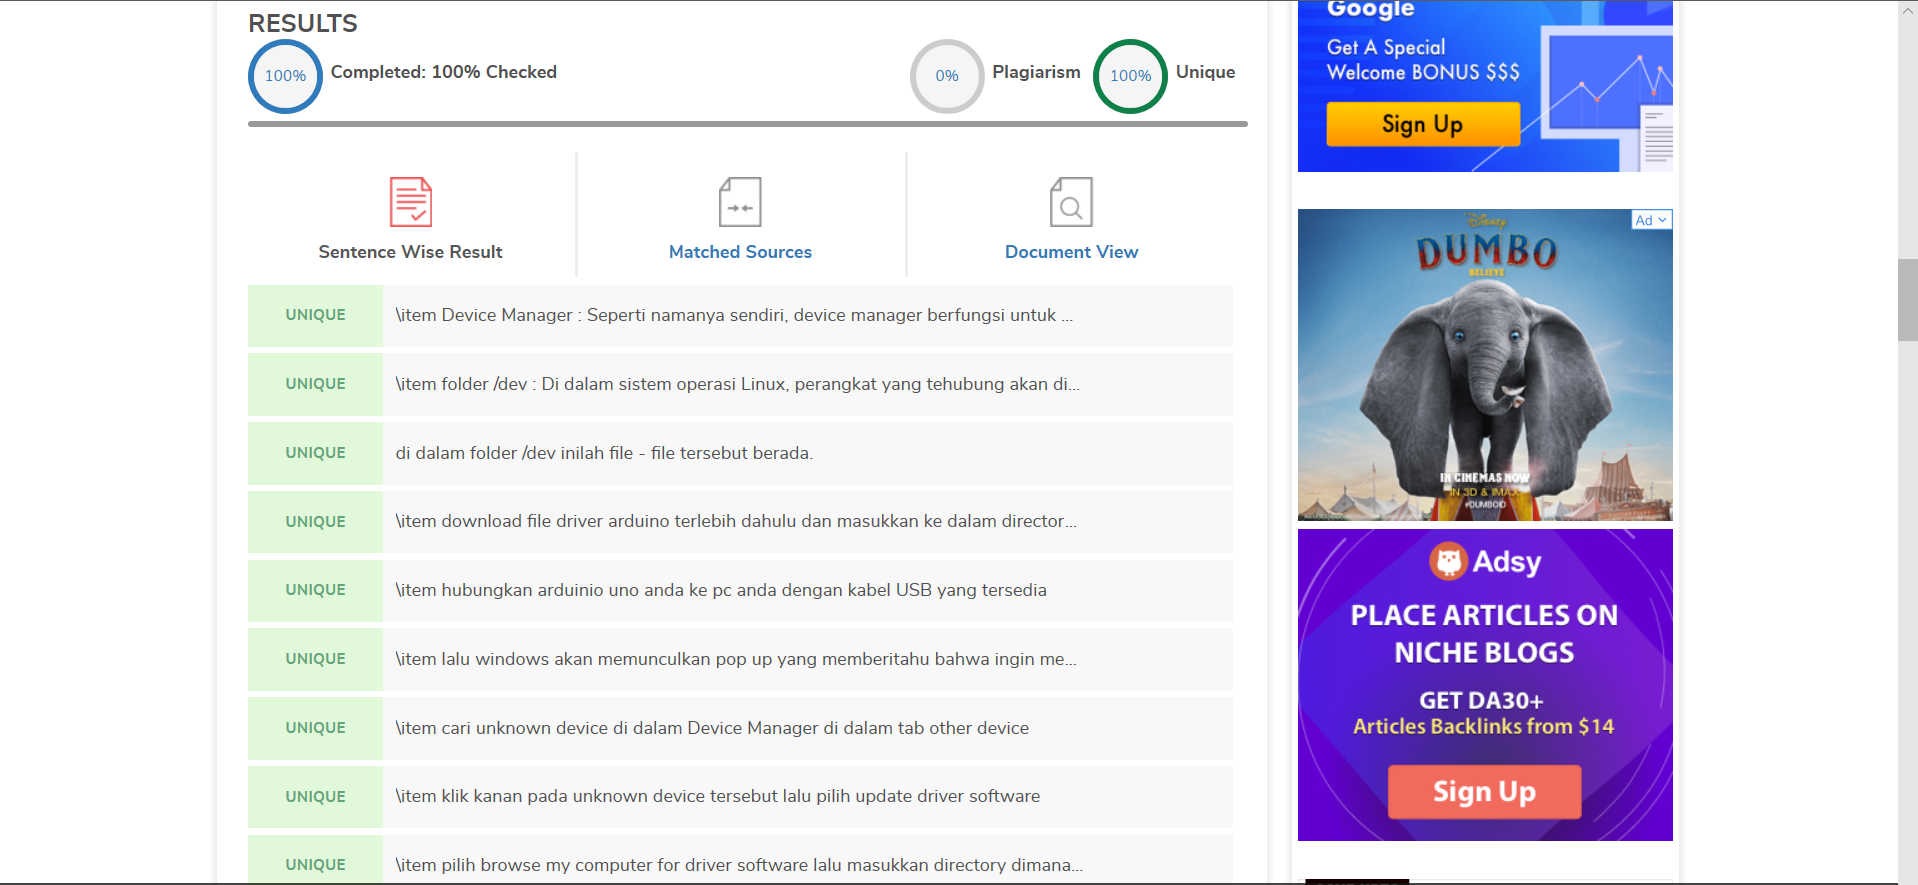
\includegraphics[width=0.5\textwidth]{figures/5/1174040/Teori/1174040_plagiat.png}}
            \caption{Cek Plagiarisme}
            \label{1174040_plagiat5}
            \end{figure}
    cek plagiarisme hagan
	

\section{Luthfi Muhammad Nabil/1174035}
\subsection{Soal 1}
Apa itu fungsi device manager di windows dan /dev di linux :
\begin{itemize}
	\item Device Manager merupakan panel kontrol pada sistem operasi windows. Pengguna dapat mengontrol dan melihat perangkat yang  telah terhubung dengan komputer dengan device manager. 
	Untuk setiap perangkat, pengguna dapat : 
		\begin{itemize}
			\item Memperbolehkan perangkat untuk beroperasi
			\item Menginformasikan sistem operasi untuk melakukan aksi pada perangkat yang tidak berfungsi
			\item Menginstall driver untuk perangkat yang terhubung
			\item Melihat informasi dari perangkat
		\end{itemize}
	\item /dev merupakan lokasi dari file untuk perangkat. /dev berfungsi untuk menampung data - data sebuah perangkat yang terhubung pada komputer. Perangkat yang dapat terhubung diantaranya perangkat penyimpanan data dan perangkat pengiriman data.
\end{itemize}

\subsection{Soal 2}
Jelaskan langkah - langkah instalasi driver dari arduino : 

Untuk instalasi driver, biasanya akan langsung terinstall jika sudah menginstall arduino IDE Seperti contoh meminta instalasi untuk arduino pada gambar \ref{PopUpInstalasi}.
\begin{figure} [ht]
		\centerline{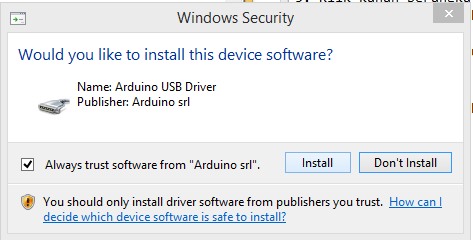
\includegraphics[width=1\textwidth]{figures/5/1174035/Teori/PopUpInstalasi.png}}
		\caption{Pop Up saat instalasi Arduino IDE}
		\label{PopUpInstalasi}
\end{figure}
Jika memang tidak ditemukan, maka ikuti langkah berikut : 
Yang dibutuhkan : 
\begin{itemize}
	\item Arduino Driver
	\item Arduino Jenis Apapun
\end{itemize}
Cara Instalasi : 
\begin{enumerate}
	\item Hubungkan arduino ke komputer (untuk arduino uno dapat menggunakan kabel type B)
	\begin{figure} [ht]
		\centerline{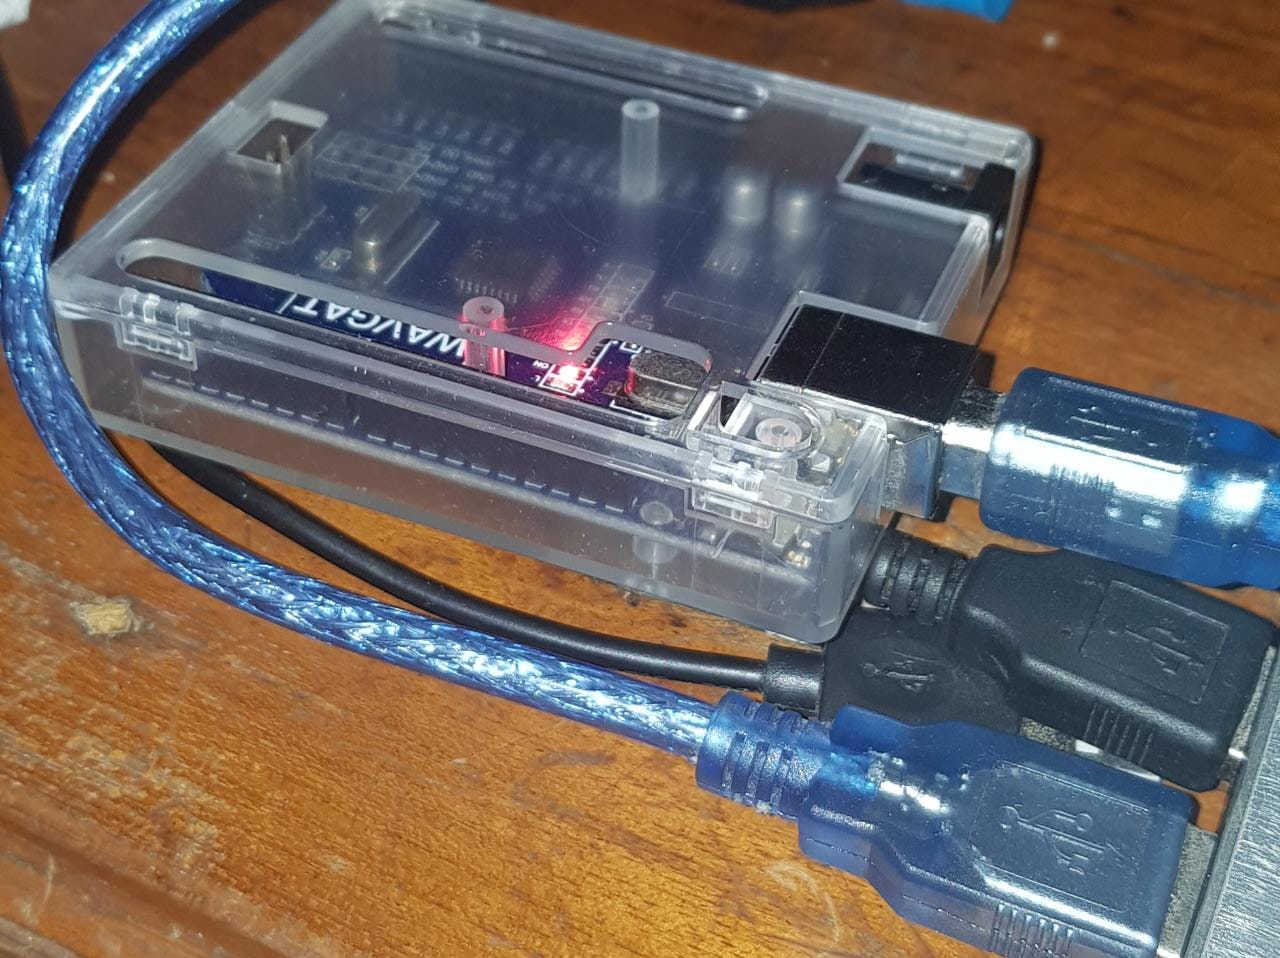
\includegraphics[width=0.6\textwidth]{figures/5/1174035/Teori/Soal1Step1.jpeg}}
		\caption{Hubungkan arduino dengan komputer}
		\label{Soal1Step1}
	\end{figure}
	\item Lalu setelah muncul popup instalasi driver akan terinstal secara otomatis. 
	\item Jika instalasi otomatis gagal, buka device manager.
		\begin{figure} [ht]
			\centerline{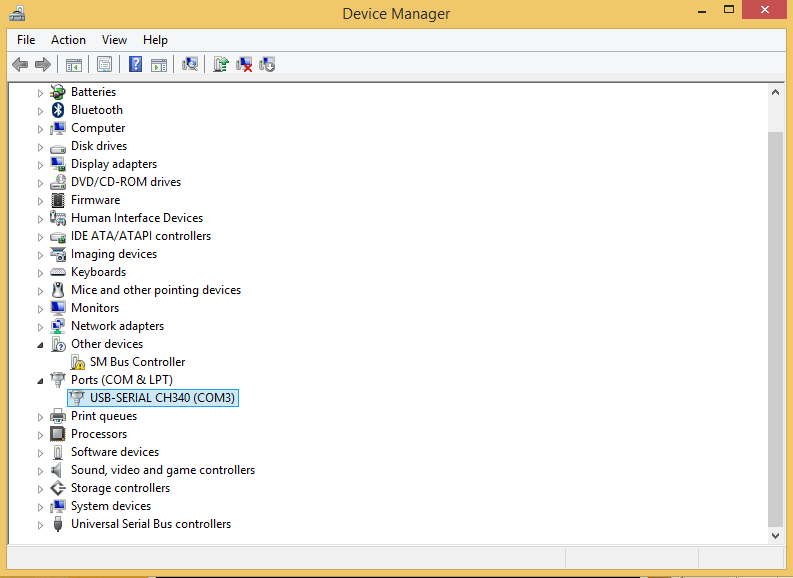
\includegraphics[width=1\textwidth]{figures/5/1174035/Teori/DeviceManagerContoh.png}}
			\caption{Tampilan Device Manager}
			\label{DevManagerContoh}
		\end{figure}
	\item Setelah device manager terbuka, cari perangkat lainnya/tidak diketahui (other device).
	\item Klik kanan perangkat yang tidak diketahui lalu pilih update driver.
	\item Pilih Cari driver (Browse my computer for driver software).
	\item Pilih lokasi driver ke driver yang telah didownload lalu klik next/ok.
	\item Setelah muncul pop up instalasi, tekan install.
	\item Instalasi Sukses
\end{enumerate}

\subsection{Soal 3}
Jelaskan bagaimana membaca baudrate dan port dari komputer yang sudah terinstall driver : 
\begin{itemize}
	\item Port : Untuk membaca port, dapat membuka file/lokasi berikut :
	
Arduino IDE : 
	\begin{figure} [ht]
			\centerline{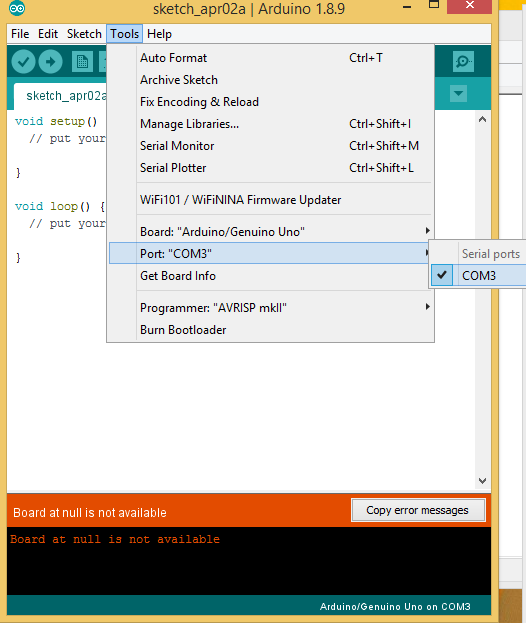
\includegraphics[width=0.6\textwidth]{figures/5/1174035/Teori/PortArduinoIDE.png}}
			\caption{Port dari Arduino IDE}
			\label{IDEPorts}
		\end{figure}
		\begin{enumerate}
			\item Buka Arduino IDE
			\item Lalu masuk ke Tools->Ports
			\item Akan muncul port serial untuk arduino seperti pada gambar \ref{IDEPorts}
		\end{enumerate}
Device Manager : 
	\begin{figure} [ht]
			\centerline{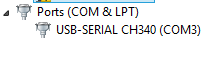
\includegraphics[width=0.6\textwidth]{figures/5/1174035/Teori/PortDeviceManager.png}}
			\caption{Port dari Device Manager}
			\label{DevManPort}
		\end{figure}
		\begin{enumerate}
			\item Buka Device Manager pada windows
			\item Cari Perangkat dengan nama Arduino
			\item Lalu lihat port berapa yang dipakai oleh Arduino Tersebut seperti pada gambar \ref{DevManPort}
		\end{enumerate}		
	\item Baudrate : Untuk melihat baudrate, dapat buka serial monitor dan cek baudrate dan tampilan fix pada tampilan serial monitor. Untuk setting default biasanya diantara 9600 dan 115200.
	\begin{figure} [ht]
			\centerline{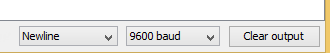
\includegraphics[width=0.6\textwidth]{figures/5/1174035/Teori/Baudrate.png}}
			\caption{Baud Rate}
			\label{BaudRate}
		\end{figure}
\end{itemize}

\subsection{Soal 4}
Sejarah PySerial : 

PySerial dibuat secara public pertama kali pada tahun 2002 dengan rilisan versi pertama 1.0. Pada saat itu PySerial sudah dapat membaca line serial dan menghapus semua isi dari serial tetapi belum dapat mengkonversi isi serial menjadi tipe data lain. PySerial juga sudah dapat melakukan Exception untuk proses yang terdapat error. Lalu pada tahun 2003 dirilis versi yang dapat mengkonversi data ke bilangan bulat, suppert terhadap python versi 2.2+ dan getter setter. Mulai pada tahun 2008, diberlakukan fitur iterasi untuk dapat mengambil seluruh data yang muncul pada serial yang diusulkan oleh Bernhard Bender. Kemudian pada tahun 2011, mulai dapat melihat daftar port yang terhubung dengan serial. Sampai akhirnya telah muncul versi 3.4 pada tahun 2017 yang sudah memperbaiki bug - bug yang ada.

\subsection{Soal 5}
Jelaskan fungsi - fungsi yang ada di pyserial.
\begin{itemize}
	\item \begin{verbatim}open()\end{verbatim} 
	Fungsi untuk membuka port serial yang terhubung
	\item \begin{verbatim}close()\end{verbatim} 
	Fungsi untuk menutup port serial yang terhubung
	\item \begin{verbatim}read(size=1) \end{verbatim}
	Fungsi untuk menentukan ukuran serial yang dapat dibaca
	\item \begin{verbatim}read\_until(expected=LF, size=None) \end{verbatim}
	Fungsi untuk membaca serial sampai sequence yang ditentukan sudah dapat.
	\item \begin{verbatim}write(data) \end{verbatim}
	Fungsi untuk menulis data ke perangkat yang terhubung.
	\item \begin{verbatim}flush() \end{verbatim}
	Fungsi untuk menghapus seluruh data yang ditampilkan di serial.
	\item \begin{verbatim}readline(size=-1) \end{verbatim}
	Untuk membaca setiap line pada tampilan yang ada pada serial
	\item \begin{verbatim}writelines(lines) \end{verbatim}
	Sama halnya dengan write yaitu untuk menulis data ke perangkat yang terhubung.
\end{itemize}
\subsection{Soal 6}
Jelaskan mengapa butuh perulangan dalam membaca serial : 

Karena perulangan digunakan untuk membaca seluruh data pada serial yang ada setiap baris. Perulangan digunakan agar data dapat muncul secara terus menerus atau realtime. Dalam konsep berjalannya sebuah microcontroller, proses yang ada akan dijalankan secara terus menerus sampai proses meminta atau processor meminta untuk memberhentikan proses tersebut sehingga jika tidak memakai perulangan, maka data yang diambil hanyalah data dimana sintaks untuk meminta data itu dipanggil. 
\subsection{Soal 7}
Jelaskan cara membuat fungsi yang menggunakan pyserial : 

Untuk membuat fungsi yang menggunakan pyserial, cukup dengan menuliskan fungsi dari pyserial dan menggunakannya dalam fungsi yang dibuat. Seperti contoh fungsi yang menggunakan PySerial : 
\lstinputlisting{src/5/1174035/Teori/chap5_1174035_teori.py}

\section{Faisal Najib Abdullah}
\subsection{Teori}
\begin{enumerate}
	\item Apa itu fungsi device manager di windows dan folder /dev di linux
	\par
		\begin{enumerate}
		    \item Device Manager : Seperti namanya sendiri, device manager berfungsi untuk menampilkan dan mengelola semua hardware yang terinstall ataupun dapat di instalasi ke dalam windows.

			\item folder /dev : Di dalam sistem operasi Linux, perangkat yang tehubung akan dianggap sebagai file. di dalam folder /dev inilah file - file  tersebut berada.
		\end{enumerate}
	
	\item Jelaskan langkah-langkah instalasi driver dari arduino
	\par
		Langkah - langkah instalasi driver arduino :
		\begin{enumerate}
			\item Pertama download file driver arduino terlebih dahulu dan masukkan ke dalam directory yang diinginkan.
			\item Hubungkan arduino uno anda ke pc anda dengan kabel USB yang tersedia.
			\item Kemudian windows akan memunculkan pop up yang memberitahu bahwa ingin menginstall dirver, tapi nanti tidak akan menemukan drivernya.
			\item Buka Device Manager dan cari unknown device di dalam Device Manager di dalam tab other device.
			\item Klik kanan pada unknown device tersebut lalu pilih update driver software
			\item Pilih browse my computer for driver software lalu masukkan directory dimana anda menyimpan driver arduino yang telah anda download tadi
			\item Setelah itu klik install dan tunggu hingga proses selesai
			\item Arduino pun sudah terbaca di pc anda 
		\end{enumerate}
	
	\item Jelaskan bagaimana cara membaca baudrate dan port dari komputer yang sudah terinstall driver
	\par
	Untuk melihat atau membaca baudrate dan port kita hanya perlu menginstall Arduino IDE, setelah itu buka menu serial monitor yang berada di tab tools. Dari sana akan terlihat baik baudrate dan port yang sedang digunakan oleh arduin anda.
	
	\item Jelaskan sejarah library pyserial
	\par
	PySerial merupakan sebuah library yang digunakan untuk komunikasi ke port serial terutama untuk mikrokontroller. PySerial pertama kali diluncurkan pada tahun 2002 yang makin berkembang dalam setiap versinya hingga tahun 2017 lalu.
	
	\item Jelaskan fungsi-fungsi apa saja yang dipakai dari library pyserial
		\begin{itemize}
			\item \begin{verbatim}serial.to_bytes(sequence)\end{verbatim} : berfungsi untuk mengubah sequence ke dalam bytes agar dapat dikirim ke dalam arduino.
			\item \begin{verbatim}stop()\end{verbatim} : untuk menghentikan pembacaan program
			\item \begin{verbatim}open()\end{verbatim} : Fungsi untuk membuka port serial yang terhubung
			\item \begin{verbatim}close()\end{verbatim} : Fungsi untuk menutup port serial yang terhubung
			\item \begin{verbatim}read(size=1) \end{verbatim} : Fungsi untuk menentukan ukuran serial yang dapat dibaca
			\item \begin{verbatim}close()\end{verbatim} : untuk menutup port dan menghentikan pembacaan program
		\end{itemize}
	
	\item Jelaskan kenapa butuh perulangan dalam tidak butuh perulangan dalam membaca serial
	\par
	Dengan menggunakan pengulangan kita dapat mengambil data berkali - kali tanpa harus mengeksekusi file python tersebut berulang - ulang. Tanpa perulangan juga penting karena dapat digunakan di saat saat tertentu seperti jika ingin mengukur suhu ruangan yang hanya dilakukan pada saat saat tertentu tidak terus menerus.
	
	\item Jelaskan bagaimana cara membuat fungsi yang mengunakan pyserial
	\par
	Untuk membuat fungsi yang menggunakan pyserial kita hanya perlu untuk menginisialisasi pembubatan funsi dengan menggunakan def namafungsi() : lalu masukkan pyserial tersebut dengan indentasi. atau cukup dengan menggunakan fungsi while loop degan menggunakan while true:
	
\end{enumerate}

\section{Ichsan Hizman Hardy}
{\Large \textbf{Teori}}
\subsection{Soal No. 1}
Apa itu fungsi device manager di windows dan folder /dev di linux?

\hfill \break
Fungsi device manager antara lain :
\begin{enumerate}
	\item Menunjukkan status suatu hardware.
	\item Menunjukkan informasi detil suatu hardware.
	\item Mengelola driver hardware
	\item Disable dan Enable hardware
	\item Mengidentifikasi konflik antar perangkat keras.
\end{enumerate}

\hfill \break
Folder /dev berisi file device, baik device blok maupun device karakter. Di dalamnya setodaknya ada file biner yang beernama MAKEDEV untuk membuat device secara manual.

\subsection{Soal No. 2}
Jelaskan langkah-langkah instalasi driver dari arduino!

\hfill \break
Berikut ini adalah langkah-langkah instalasi driver dari Arduino UNO di Windows:

\begin{enumerate}
	\item Hubungkan sistem minimun Arduino Uno ke komputer dengan kabel USB type B (kabel Printer).
	\item Lalu pada bagian kanan didesktop PC anda, akan muncul popup “Installing device driver software”.
	\item SIstem operasi Windows tidak menyediakan driver untuk Arduino Uno.
	\item Buka Device Manager, caranya pada bagian Search Program and Files lalu ketikkan “device manager” (tanpa tanda petik). Kemudian bagian Control Panel akan muncul halaman Device Manager, selanjutnya klik untuk menjalankan.
	\item Cari yang bernama Unknown device yang berada pada bagian Other device, biasanya ada tanda seru berwarna kuning, itu disebabkan karena penginstallan tidak berjalan dengan sempurna.
	\item Klik kanan pada “Unknown device” kemudian pilih Update Driver Software.
	\item Pilih Browse my computer for driver software.
	\item Arahkan lokasi folder ke folder ..arduino-1.0.5 drivers. Pastikan check-box lalu centang include subfolders. Klik Next untuk melanjutkan instalasi driver.
	\item Kemudian lanjutkan dengan mengklik Install pada tampilan Windows Security.
	\item Jika instalasi driver berhasil maka akan muncul Windows has successfully updated your driver software.
	\item Perhatikan dan ingat nama COM Arduino Uno, karena nama COM ini yang akan digunakan untuk meng-upload program nantinya.
\end{enumerate}

\subsection{Soal No. 3}
Jelaskan bagaimana cara membaca baudrate dan port dari komputer yang sudah terinstall driver!

\hfill \break
\textbf{Membaca Port dari Komputer}

\begin{enumerate}
	\item Hubungkan modul TX-RX serial dengan komputer melalui serial port menggunakan DB9 cable extension.
	\item Buka Hyper Terminal dengan menekan start kemudian All progams lalu Accessories kemudian Communications lalu Hyper Terminal.
	\item Ketik nama untuk Connection Description, misal coba, kemudian tekan OK.
	\item Pada Connect to, pilihlah COM port yang dipakai di Connect using, kemudian tekan OK.
	\item Masukkan nilai-nilai port settingnya, sesuai dengan DCE-nya. Kemudian tekan OK.
\end{enumerate}



\subsection{Soal No. 4}
Jelaskan sejarah library pyserial!

\hfill \break
PySerial adalah library/modul Python siap-pakai dan gratis yang dibuat untuk memudahkan kita dalam membuat program komunikasi data serial RS232 dalam bahasa Python.
Jika modul USB-2REL dapat kita kontrol dengan mudah menggunakan Python dan PyUSB (lihat pembahasannya di sini dan di sini), maka modul SER-2REL juga dapat kita kontrol dengan mudah menggunakan Python dengan bantuan modul PySerial.

\subsection{Soal No. 5}
Jelaskan fungsi-fungsi apa saja yang dipakai dari library pyserial!

\hfill \break
Fungsi-fungsi yang dipakai dari library PySerial, yaitu:
\begin{enumerate}
	\item Serial - fungsi ini untuk membuka port serial.
	\item write(data) - fungsi ini menulis data lewat port serial.
	\item readline() - fungsi ini membaca sebuah string dari port serial.
	\item read(size) - fungsi ini untuk membaca jumlah byte dari port serial.
	\item close() - fungsi ini untuk menutup port serial.
\end{enumerate}

\subsection{Soal No. 6}
Jelaskan kenapa butuh perulangan dan tidak butuh perulangan dalam membaca serial!

\hfill \break
Pada saat membaca serial di Arduino diperlukan perulangan agar bisa membaca data secara berulang kali sehingga data yang muncul banyak. Sedangkan apabila tidak membutuhkan perulangan maka Arduino hanya akan membaca data sekali saja.

\subsection{Soal No. 7}
Jelaskan bagaimana cara membuat fungsi yang mengunakan pyserial!

\hfill \break
Fungsi yang berada pada Python, dibuat dengan nama kata kunci def kemudian diikuti dengan nama fungsinya pada pyhton.
Seperti halnya dengan blok kode yang lain, kita juga harus memberikan identasi untuk menuliskan isi fungsi.

\section{Dika Sukma Pradana 1174050}
	\subsection{Pemahaman Teori}
		\begin{enumerate}
			\item Apa itu fungsi device manager di windows dan folder /dev di linux?
				\par
				Device manager merupakan perangkat lunak untuk menampilkan seluruh perangkat keras yang di-inisialisasi atau dikenali oleh sistem operasi Windows. Device Manager membantu dalam mengelola atau me-manage semua perangkat keras yang terpasang dan terdeteksi dalam sistem Windows. Perangkat keras tersebut bisa berupa harddisk, kartu VGA, sound, keyboard, perangkat USB dan lain-lainnya.
				
				\par
				Fungsi device manager antara lain :
					\begin{itemize}
						\item Menunjukkan status mengenai suatu perangkat keras.
						\item Menunjukkan informasi detail mengenai suatu perangkat keras.
						\item Mengelola driver perangkat keras.
						\item Menonaktifkan dan mengaktifkan perangkat keras.
						\item Mengidentifikasi konflik antar perangkat keras.
						\item Memberitahukan terjadinya masalah pada perangkat keras.
					\end{itemize}

				\par
				Folder /dev merupakan representasi dari drive yang terhubung ke sistem operasi Linux dan oleh sistem dianggap sebagai file-file direktori. Biasanya sering ditampilkan direktori seperti /dev/sda1 yang mewakili Drive SATA pertama dalam sistem.
				
			\item Jelaskan langkah-langkah instalasi driver dari arduino!
				\begin{enumerate}
					\item Hubungkan sistem minimun Arduino Uno ke komputer dengan kabel USB type B (kabel Printer).
					\item Lalu pada bagian kanan didesktop PC anda, akan muncul popup Installing device driver software seperti pada gambar dibawah ini.
					\item Windows tidak menyediakan driver arduino, jadi kita harus menginstal secara manual.
					\item Buka Device Manager, klik untuk menjalankan.
					\item Cari Unknown device pada bagian Other device, bila terdapat tanda seru berarti peroses penginstalan belum berhasil sepenuhnya.
					\item Klik kanan pada Unknown device lalu pilih Update Driver Software.
					\item Pilih Browse my computer for driver software.
					\item Arahkan lokasi folder ke folder ..arduino1.0.5 drivers. Pastikan checkbox lalu centang include subfolders. Klik Next untuk melanjutkan instalasi driver.
					\item Kemudian lanjutkan dengan mengklik Install pada tampilan Windows Security.
					\item Jika instalasi driver berhasil maka akan muncul Windows has successfully updated your driver software.
					\item Perhatikan dan ingat nama COM Arduino Uno, karena nama COM ini yang akan digunakan untuk meng-upload program nantinya.
				\end{enumerate}
				
			\item Jelaskan bagaimana cara membaca baudrate dan port dari komputer yang sudah terinstall driver!
				\begin{itemize}
					\item Membaca Baudrate dari Komputer
						\begin{enumerate}
							\item Pertama buka Start. Cari Device Manager, lalu klik.
							\item Kemudian pilih Ports (COM \& LPT).
							\item Klik dua kali pada COM yang terhubung.
							\item Pilih tab Port Settings, lalu lihat di Bit per second.
						\end{enumerate}
					\item Membaca Port dari Komputer
						\begin{enumerate}
							\item Pertama buka Start. Cari Device Manager, lalu klik.
							\item Kemudian pilih Ports (COM \& LPT).
							\item Port dari Arduino telah terbaca oleh PC.
						\end{enumerate}
				\end{itemize}
							
			\item Jelaskan sejarah library pyserial!
			\par 
			PySerial adalah paket Python yang menfasilitasi komunikasi serial antara PC dengan perangkat keras eksternal. PySerial menyediakan antarmuka untuk berkomunikasi melalui protokol komunikasi serial. Komunikasi serial adalah salah satu protokol komunikasi komputer tertua. Protokol komunikasi serial mendahului spesifikasi USB yang digunakan oleh komputer dan perangkat keras lain seperti mouse, keyboard, dan webcam. USB adalah singkatan dari Universal Serial Bus. USB dan dibangun di atas dan memperluas antarmuka komunikasi serial asli.
			
			\item Jelaskan fungsi-fungsi apa saja yang dipakai dari library pyserial!
			Fungsi-fungsi yang dipakai dari library PySerial, yaitu:
				\begin{itemize}
					\item \begin{verbatim} serial \end{verbatim} : fungsi ini untuk membuka port serial.
					\item \begin{verbatim} write(data) \end{verbatim} : fungsi ini menulis data lewat port serial.
					\item \begin{verbatim} readline() \end{verbatim} : fungsi ini membaca sebuah string dari port serial.
					\item \begin{verbatim} read(size) \end{verbatim} fungsi ini untuk membaca jumlah byte dari port serial.
					\item \begin{verbatim} close() \end{verbatim} : fungsi ini untuk menutup port serial.
				\end{itemize}
			
			\item Jelaskan kenapa butuh perulangan dan tidak butuh perulangan dalam membaca serial!
			\par
			Perualangan dalam bahasa pemrograman berfungsi menyuruh komputer melakukan sesuatu secara berulang-ulang. Terdapat dua jenis perualangan dalam bahasa pemrograman python, yaitu perulangan dengan for dan while. Perulangan for disebut counted loop (perulangan yang terhitung), sementara perulangan while disebut uncounted loop (perulangan yang tak terhitung). Perulangan for biasanya digunakan untuk mengulangi kode yang sudah dipastikan banyak perulangannya. Sedangkan while untuk perulangan yang ditentukan dan belum pasti banyaknya. Perulangan diperlukan agar dapat membaca data secara berulang kali sehingga data yang muncul lebih dari satu.  Sedangkan apabila tidak memakai perulangan maka data akan terbaca satu kali saja.
			
			\item Jelaskan bagaimana cara membuat fungsi yang mengunakan pyserial!
				\begin{verbatim}			
					import serial

					def baca():
						ser = serial.Serial("COM4",9600)
						baca = ser.readline()
						print(baca)

					baca()
				\end{verbatim}
				
			\item Plagiarism
			\begin{figure}[H]
				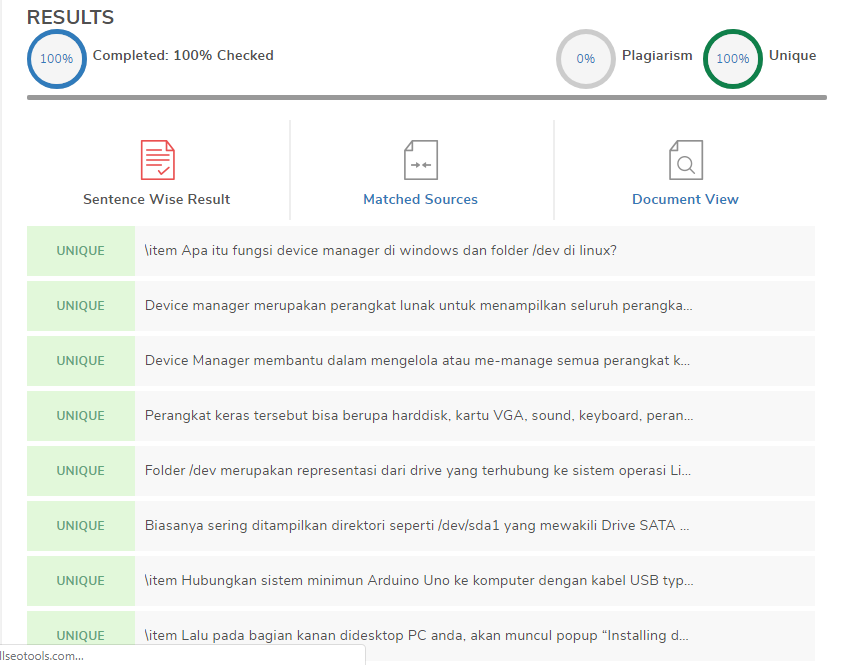
\includegraphics[width=10cm]{figures/5/1174050/Teori/plagiarism.png}
				\centering
				\caption{Hasil Scan Plagiarism}
			\end{figure}
			
		\end{enumerate}
%PRAKTEK
\chapter{Praktek Library CSV dan Pandas}
\section{Faisal Najib Abdullah 1174042}
\subsection{Keterampilan Pemrograman}
\begin{enumerate}
	\item Buatlah fungsi file terpisah dengan nama NPM realtime.py untuk mendapatkan data langsung dari arduino
	\lstinputlisting[caption = Fungsi untuk mendapatkan data dari Arduino., firstline=1, lastline=7]{src/5/1174042/Praktek/1174042_realtime.py}

	\begin{figure}[H]
		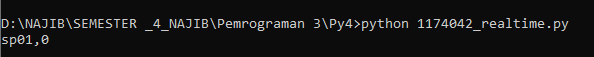
\includegraphics[width=12cm]{figures/5/1174042/Praktek/1.png}
		\centering
		\caption{Hasil dari pembacaan fungsi untuk mendapatkan data dari Arduino.}
	\end{figure}
	
	\item Buatlah fungsi file terpisah dengan nama NPM save.py untuk mendapatkan data langsung dari arduino dengan looping
	\lstinputlisting[caption = Fungsi untuk mendapatkan data langsung dari Arduino dengan looping., firstline=1, lastline=8]{src/5/1174042/Praktek/1174042_save.py}

	\begin{figure}[H]
		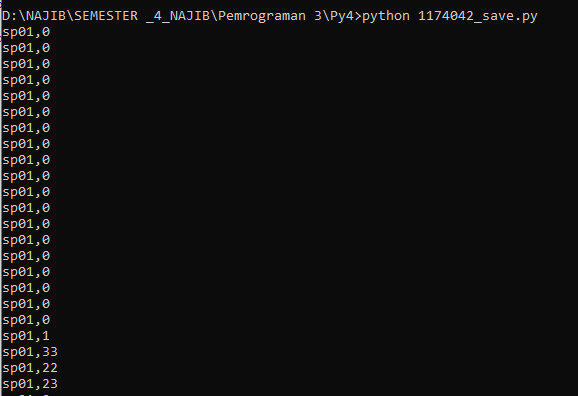
\includegraphics[width=12cm]{figures/5/1174042/Praktek/2.png}
		\centering
		\caption{Hasil dari pembacaan fungsi untuk mendapatkan data dari Arduino dengan looping.}
	\end{figure}
	
	\item Buatlah fungsi file terpisah dengan nama NPM realtime.py untuk mendapatkan data dari arduino dan langsung ditulis kedalam file csv
	\lstinputlisting[caption = Fungsi untuk mendapatkan data dari Arduino dan langsung ditulis kedalam file CSV., firstline=9, lastline=23]{src/5/1174042/Praktek/1174042_realtime.py}

	\begin{figure}[H]
		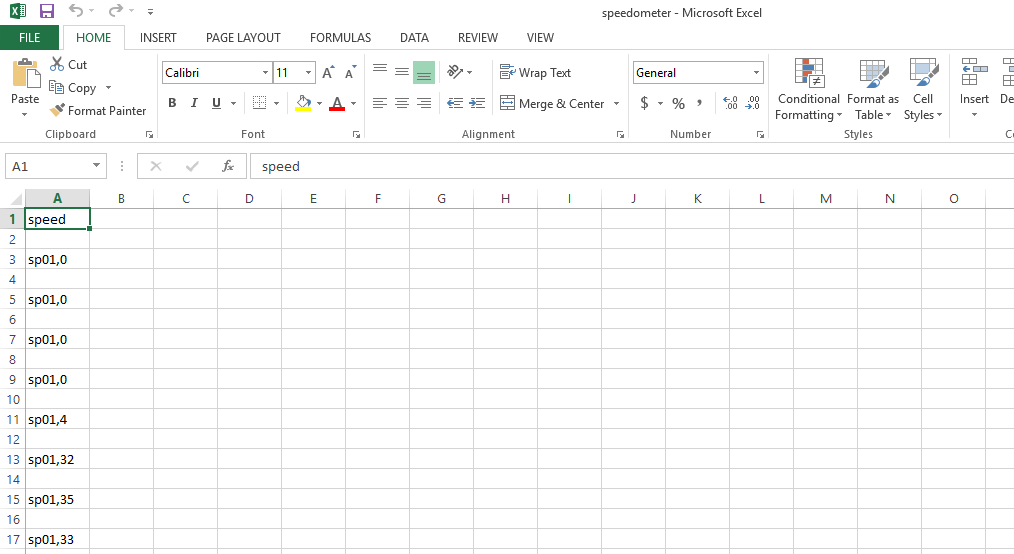
\includegraphics[width=12cm]{figures/5/1174042/Praktek/3.png}
		\centering
		\caption{Hasil dari pembacaan fungsi untuk mendapatkan data dari Arduino dan langsung ditulis kedalam file CSV.}
	\end{figure}
	
	\item Buatlah fungsi file terpisah dengan nama NPM csv.py untuk membaca file csv hasil arduino dan mengembalikan ke fungsi
	\lstinputlisting[caption = Fungsi untuk membaca file CSV hasil Arduino dan mengembalikan fungsi., firstline=1, lastline=9]{src/5/1174042/Praktek/1174042_csv.py}

	\begin{figure}[H]
		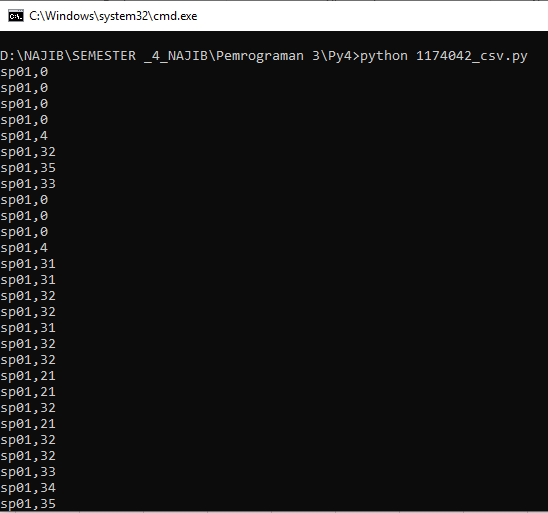
\includegraphics[width=12cm]{figures/5/1174042/Praktek/4.png}
		\centering
		\caption{Hasil dari pembacaan fungsi untuk membaca file csv hasil arduino dan mengembalikan fungsi.}
	\end{figure}
	
\end{enumerate}

\subsection{Penanganan Error}
Tuliskan  peringatan  error  yang  didapat  dari  mengerjakan  praktek  kelima  ini, dan  jelaskan  cara  penanganan  error  tersebut.   dan  Buatlah  satu  fungsi  yang menggunakan try except untuk menanggulangi error tersebut.

\hfill \break
Peringatan error di praktek kelima ini, yaitu:
\begin{itemize}
	\item Syntax Errors
	Syntax Errors adalah suatu keadaan saat kode python mengalami kesalahan penulisan. Solusinya adalah memperbaiki penulisan kode yang salah.
	
	\item Name Error
	NameError adalah exception yang terjadi saat kode melakukan eksekusi terhadap local name atau global name yang tidak terdefinisi. Solusinya adalah memastikan variabel atau function yang dipanggil ada atau tidak salah ketik.
	
	\item Type Error
	TypeError adalah exception yang akan terjadi apabila pada saat dilakukannya eksekusi terhadap suatu operasi atau fungsi dengan type object yang tidak sesuai. Solusi dari error ini adalah mengkoversi varibelnya sesuai dengan tipe data yang akan digunakan.
\end{itemize}

\hfill \break
Fungsi yang menggunakan try except untuk menanggulangi error.

\lstinputlisting[caption = Fungsi untuk menanggulangi error menggunakan Try Except., firstline=1, lastline=16]{src/5/1174042/Praktek/1174042.py}

\begin{figure}[H]
	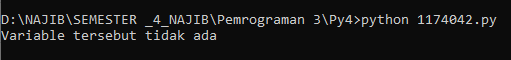
\includegraphics[width=12cm]{figures/5/1174042/Praktek/5.png}
	\centering
	\caption{Hasil pembacaan fungsi untuk menanggulangi error menggunakan Try Except.}
\end{figure}

\section{Hagan Rowlenstino/1174040}
	\subsection{Soal 1} 
		membuat fungsi untuk mendapatkan data langsung dari arduino. disini saya menggunakan arduino dengan servo. disini saya akan menginputkan data berupa angka untuk menambahkan berapa lama cervo kembali dari letak yang di tentukan ke letak awal.

	\lstinputlisting[firstline=1, lastline=13]{src/5/1174040/Praktek/chap5_1174040_realtime.py}

	\subsection{Soal 2}
	membuat fungsi untuk mendapatkan data langsung dari arduino dengan looping. disini saya menggunakan arduino dengan servo. disini saya akan menginputkan data berupa angka untuk menambahkan berapa lama cervo kembali dari letak yang di tentukan ke letak awal.

	\lstinputlisting{src/5/1174040/Praktek/chap5_1174040_save.py}

	\subsection{Soal 3}
	membuat fungsi untuk mendapatkan data langsung dari arduino lalu me write data tersebut ke dalam file csv. disini saya menggunakan arduino dengan servo. disini saya akan menginputkan data berupa angka untuk menambahkan berapa lama cervo kembali dari letak yang di tentukan ke letak awal. Nilai inputan tersebutlah yang saya  write ke dalam file 1174040\_realtime2.csv

	\lstinputlisting[firstline=15, lastline=26]{src/5/1174040/Praktek/chap5_1174040_realtime.py}

	\subsection{Soal 4}
	
	fungsi untuk membaca csv yang brisikan data dari arduino tadi :

	\lstinputlisting{src/5/1174040/Praktek/chap5_1174040_csv.py}

	\subsection{Penanganan Error}
	Disini saya mendapatkan Error yaitu FileNotFoundError dimana ada kesalahan saat menginputkan nama file yang akan digunakan, untuk penanganannya yaitu dengan cara menginputkan nama file yang benar 

	\lstinputlisting{src/5/1174040/Praktek/chap5_1174040_err.py}
	
\section{Irvan Rizkiansyah/1174043}
	\subsection{Nomor 1}
		\lstinputlisting[firstline=12, lastline=20]{src/5/1174043/Praktek/chap5_1174043_realtime.py}
		
	\subsection{Nomor 2}
		\lstinputlisting[firstline=8, lastline=22]{src/5/1174043/Praktek/chap5_1174043_simpan.py}
	
	\subsection{Nomor 3}
		\lstinputlisting[firstline=22, lastline=33]{src/5/1174043/Praktek/chap5_1174043_realtime.py}
	
	\subsection{Nomor 4}
		\lstinputlisting[firstline=8, lastline=16]{src/5/1174043/Praktek/chap5_1174043_csv.py}
		
	\subsection{Penanganan Error}
		\lstinputlisting[firstline=8, lastline=19]{src/5/1174043/Praktek/chap5_1174043_error.py}
		
\section{Luthfi Muhammad Nabil/1174035}
	\subsection{Soal 1}
	Membuat fungsi untuk mengambil data langsung dari arduino. 
	\lstinputlisting[firstline=1, lastline=5]{src/5/1174035/Praktek/chap5_1174035_realtime.py}
	\begin{figure}[H]
		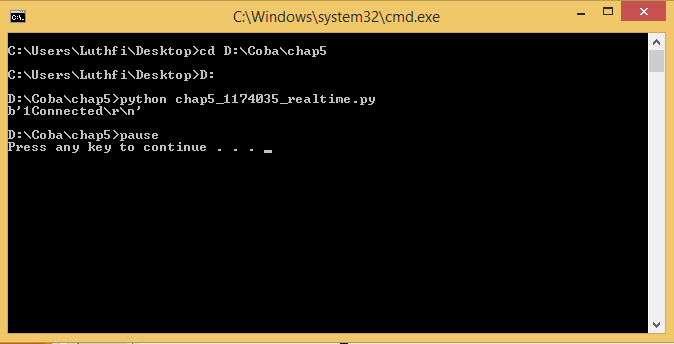
\includegraphics[width=12cm]{figures/5/1174035/Praktek/ReadNonLoop.png}
		\centering
		\caption{Hasil dari Ambil Data tanpa perulangan}
	\end{figure}
	\subsection{Soal 2}
	Membuat fungsi untuk mengambil data langsung dari arduino dengan looping. 
	\lstinputlisting{src/5/1174035/Praktek/chap5_1174035_save.py}
	\begin{figure}[H]
		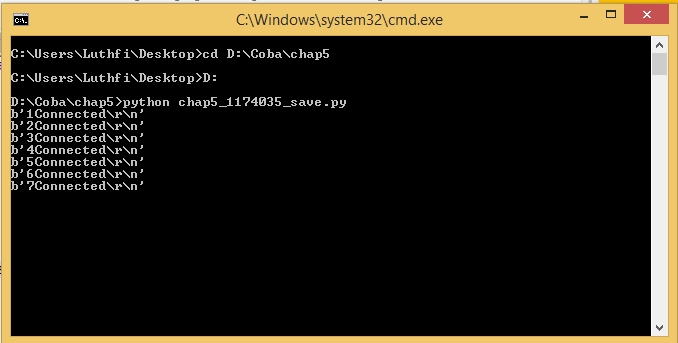
\includegraphics[width=12cm]{figures/5/1174035/Praktek/ReadLoop.png}
		\centering
		\caption{Hasil dari Ambil Data dengan perulangan}
	\end{figure}
	\subsection{Soal 3}
	Membuat fungsi untuk mengambil data langsung dari arduino lalu me write data tersebut ke dalam file csv.
	\lstinputlisting[firstline=7]{src/5/1174035/Praktek/chap5_1174035_realtime.py}
	\begin{figure}[H]
		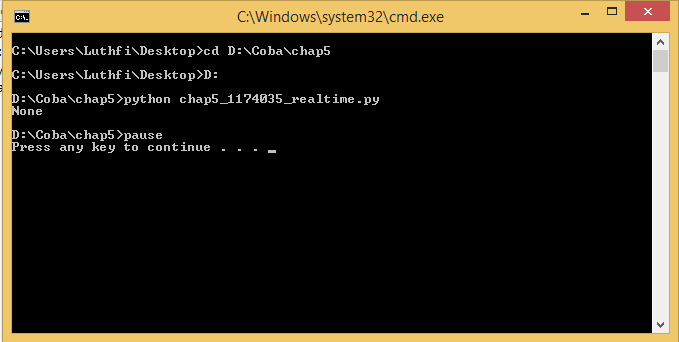
\includegraphics[width=12cm]{figures/5/1174035/Praktek/WriteCSV.png}
		\centering
		\caption{Menulis data dari serial ke file CSV}
	\end{figure}
	\begin{figure}[H]
		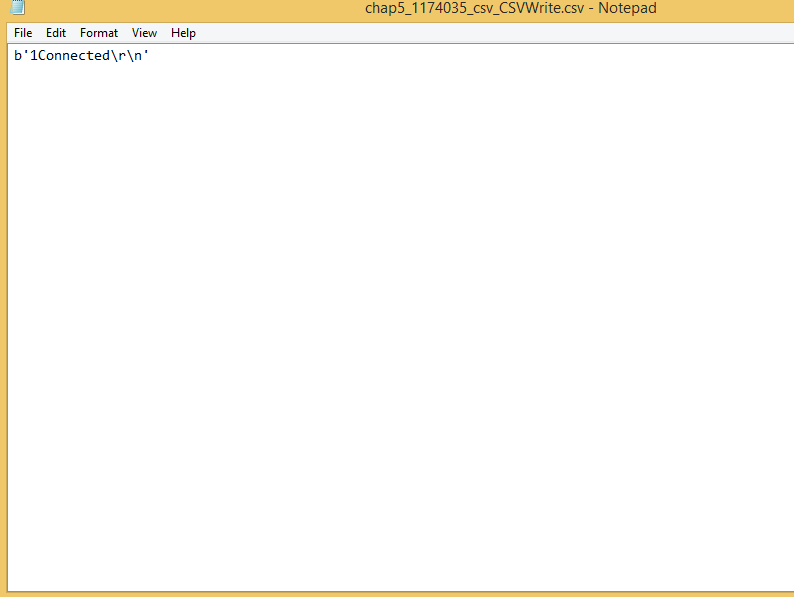
\includegraphics[width=12cm]{figures/5/1174035/Praktek/HasilCSV.png}
		\centering
		\caption{Hasil Tulis CSV dengan ambilan tanpa loop}
	\end{figure}
	\subsection{Soal 4}
	Fungsi untuk membaca csv yang berisikan data dari isi serial arduino yang dibaca sebelumnya :
	\lstinputlisting{src/5/1174035/Praktek/chap5_1174035_save.py}
	
	\subsection{Penanganan Error}
	Error yang didapat : Serial Exception
	Definisi : Serial Exception terjadi saat koneksi antara serial dan komputer terjadi masalah atau tidak dapat berkomunikasi. Untuk menangani error tersebut dapat menggunakan Try Except.
	
	Pemakaian : \lstinputlisting{src/5/1174035/Praktek/chap5_1174035_error.py}
	
	Hasil (Saat Error) dapat dilihat pada gambar \ref{Error_1174035}
	\begin{figure}[H]
		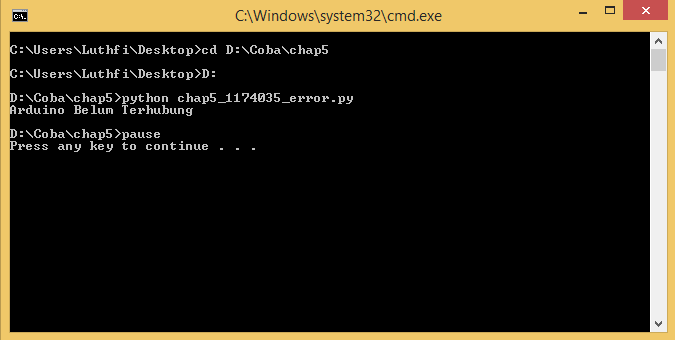
\includegraphics[width=12cm]{figures/5/1174035/Praktek/Error.png}
		\centering
		\caption{Hasil dari Error}
		\label{Error_1174035}
	\end{figure}
	
	\section{Dika Sukma Pradana 1174050}
\subsection{Keterampilan Pemrograman}
\begin{enumerate}
	\item Buatlah fungsi file terpisah dengan nama NPM realtime.py untuk mendapatkan data langsung dari arduino
	\lstinputlisting[caption = Fungsi untuk mendapatkan data dari Arduino., firstline=1, lastline=7]{src/5/1174050/Praktek/1174050_realtime.py}

	\begin{figure}[H]
		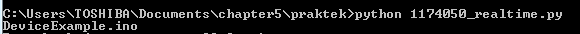
\includegraphics[width=12cm]{figures/5/1174050/Praktek/realtime.png}
		\centering
		\caption{Hasil dari pembacaan fungsi untuk mendapatkan data dari Arduino.}
	\end{figure}
	
	\item Buatlah fungsi file terpisah dengan nama NPM save.py untuk mendapatkan data langsung dari arduino dengan looping
	\lstinputlisting[caption = Fungsi untuk mendapatkan data langsung dari Arduino dengan looping., firstline=1, lastline=8]{src/5/1174050/Praktek/1174050_save.py}

	\begin{figure}[H]
		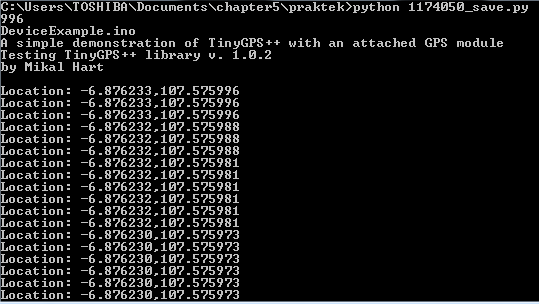
\includegraphics[width=12cm]{figures/5/1174050/Praktek/save.png}
		\centering
		\caption{Hasil dari pembacaan fungsi untuk mendapatkan data dari Arduino dengan looping.}
	\end{figure}
	
	\item Buatlah fungsi file terpisah dengan nama NPM realtime.py untuk mendapatkan data dari arduino dan langsung ditulis kedalam file csv
	\lstinputlisting[caption = Fungsi untuk mendapatkan data dari Arduino dan langsung ditulis kedalam file CSV., firstline=9, lastline=23]{src/5/1174050/Praktek/1174050_realtime.py}

	\begin{figure}[H]
		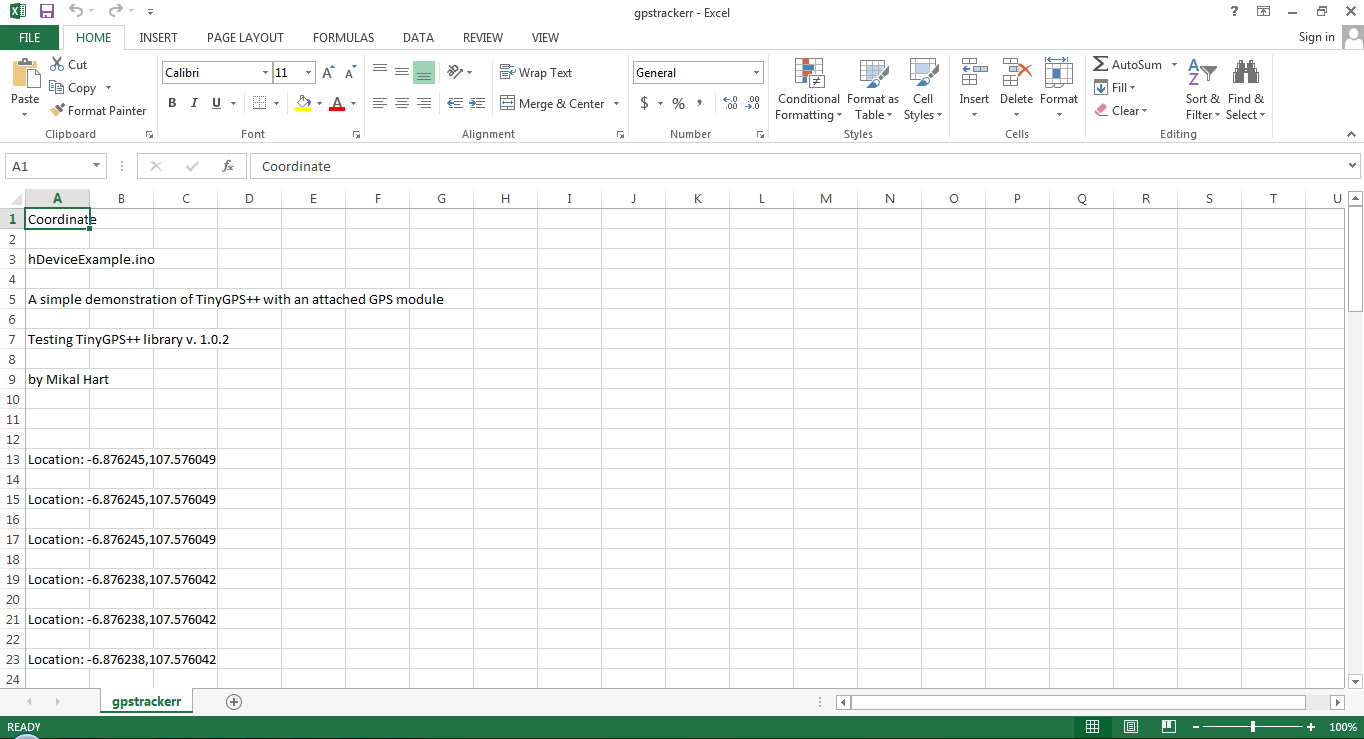
\includegraphics[width=12cm]{figures/5/1174050/Praktek/csvfile.png}
		\centering
		\caption{Hasil dari pembacaan fungsi untuk mendapatkan data dari Arduino dan langsung ditulis kedalam file CSV.}
	\end{figure}
	
	\item Buatlah fungsi file terpisah dengan nama NPM csv.py untuk membaca file csv hasil arduino dan mengembalikan ke fungsi
	\lstinputlisting[caption = Fungsi untuk membaca file CSV hasil Arduino dan mengembalikan fungsi., firstline=1, lastline=9]{src/5/1174050/Praktek/1174050_csv.py}

	\begin{figure}[H]
		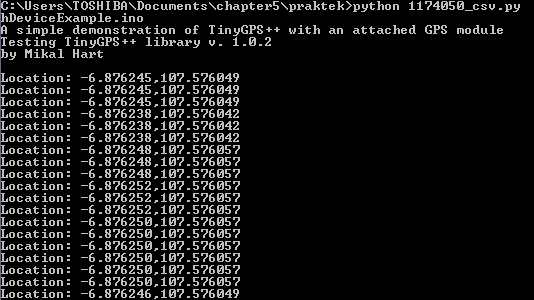
\includegraphics[width=12cm]{figures/5/1174050/Praktek/csvv.png}
		\centering
		\caption{Hasil dari pembacaan fungsi untuk membaca file csv hasil arduino dan mengembalikan fungsi.}
	\end{figure}
	
\end{enumerate}

\subsection{Penanganan Error}
Tuliskan  peringatan  error  yang  didapat  dari  mengerjakan  praktek  kelima  ini, dan  jelaskan  cara  penanganan  error  tersebut.   dan  Buatlah  satu  fungsi  yang menggunakan try except untuk menanggulangi error tersebut.

\hfill \break
Peringatan error di praktek kelima ini, yaitu:
\begin{itemize}
	\item Syntax Errors
	Syntax Errors adalah suatu keadaan saat kode python mengalami kesalahan penulisan. Solusinya adalah memperbaiki penulisan kode yang salah.
	
	\item Name Error
	NameError adalah exception yang terjadi saat kode melakukan eksekusi terhadap local name atau global name yang tidak terdefinisi. Solusinya adalah memastikan variabel atau function yang dipanggil ada atau tidak salah ketik.
	
	\item Type Error
	TypeError adalah exception yang akan terjadi apabila pada saat dilakukannya eksekusi terhadap suatu operasi atau fungsi dengan type object yang tidak sesuai. Solusi dari error ini adalah mengkoversi varibelnya sesuai dengan tipe data yang akan digunakan.
\end{itemize}

\hfill \break
Fungsi yang menggunakan try except untuk menanggulangi error.

\lstinputlisting[caption = Fungsi untuk menanggulangi error menggunakan Try Except., firstline=1, lastline=16]{src/5/1174050/Praktek/1174050.py}

\begin{figure}[H]
	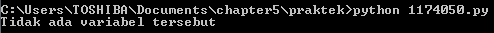
\includegraphics[width=12cm]{figures/5/1174050/Praktek/error.png}
	\centering
	\caption{Hasil pembacaan fungsi untuk menanggulangi error menggunakan Try Except.}
\end{figure}
	

\chapter{Library CSV dan Pandas}
\section{Hagan Rowlenstino/1174040}
	\subsection{Soal 1}
	library matplotlib adalah sebuah library untuk memplotting 2 Dimensi yang output nya adalah gambar publikasi yang bermutu di banyak format hardocpy serta lingkungan interaktif berbagai platform

	\subsection{Soal 2}
	untuk membuat sumbu x dan y :
	\lstinputlisting{src/6/1174040/Teori/chap6_1174040_2.py}

	\subsection{Soal 3}
	\begin{itemize}
		\item PLot Garis :

		\lstinputlisting[firstline=8, lastline=13]{src/6/1174040/Teori/chap6_1174040_3.py}

		\item Plot Sebaran

		\lstinputlisting[firstline=15, lastline=18]{src/6/1174040/Teori/chap6_1174040_3.py}

		\item Plot Batang / Histogram

		\lstinputlisting[firstline=20, lastline=23]{src/6/1174040/Teori/chap6_1174040_3.py}

		\item Pie

		\lstinputlisting[firstline=26, lastline=35]{src/6/1174040/Teori/chap6_1174040_3.py}

	\end{itemize}

	\subsection{Soal 4}
	\begin{itemize}
		\item Legend : Penjelasan garis beserta contoh dari garis yang dijelaskan tersebut. untuk membuat legend dapat menggunakan sintaks berikut :

		\begin{verbatim} legend('legend grafik1',…,'legend grafikN','Nilai Pos') \end{verbatim}
		
		\item Label : Memberikan penamaan untuk skala(sumbu) yang kita buat. untuk menambahkan label, kita dapat menggunakan sintaks berikut :

		\begin{verbatim} 
		xlabel(‘teks horizontal axis’)

		ylabel(‘teks vertikal axis’)
		\end{verbatim}
	\end{itemize}

	\subsection {Soal 5}
	Subplot pada matplotlib berfungsi untuk membuat banyak plot grafik dalam satu figure saja.
	dimana  subplot dapat kita definisikan sebagai berikut :
	
	\begin{verbatim} subplot(m,n,i) 
	\end{verbatim}
	Dimana m adalah tinggi nya, n adalah lebar nya dan i adalah urutan penempatannya.
	Untuk membuat 9 subplot dapat dilihati dari contoh dibawah ini :

	\lstinputlisting{src/6/1174040/Teori/chap6_1174040_5.py}

	\begin{figure}[ht]
            \centerline{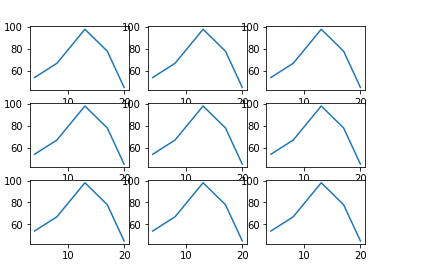
\includegraphics[width=0.5\textwidth]{figures/6/1174040/Teori/1174040_no5.png}}
            \caption{No. 5}
            \label{1174040_chap6_no5}
            \end{figure}

	\subsection{Soal 6}
	color yang dapat digunakan adalah red(r),blue(b),green(g),cyan(c),magenta(m),yellow(y),black(k),white(w)

	\subsection{Soal 7}
	fungsi Hist digunakan untuk membuat histogram yang berfungsi untuk menampilkan frekuensi data dengan menggunakan grafik batang

	\lstinputlisting{src/6/1174040/Teori/chap6_1174040_hist.py}

	\begin{figure}[ht]
            \centerline{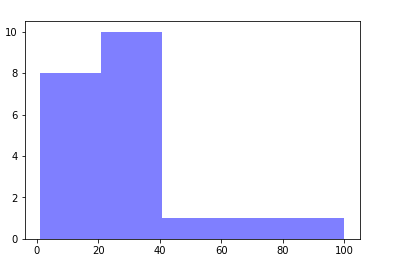
\includegraphics[width=0.5\textwidth]{figures/6/1174040/Teori/1174040_no7.png}}
            \caption{No. 7}
            \label{1174040_chap6_no7}
            \end{figure}

	\subsection{Soal 8}
	\begin{itemize}
		\item Labels : Untuk memberi penamaan terhadap setiap potongan dari pie
		\item colors : Untuk memberikan warna spesifik terhadap potongan potongan pie, jika tidak diberi warna maka dia akan menggambi warna dari pie yang telah berjalan
		\item startangle : Untuk menetapkan dari sudut mana grafik tersebut akan dimulai
		\item shadow : untuk memberikan efek bayangan di bawah pie maupun potongannya
		\item explode : untuk menentukan seerapa jauh pemisahkan potongan pie dari potongan - potongan lainnya
		\item autopct : untuk memberikan nilai atau skalal numeric pada label didalam potongan pie . seperti mengubah dari 10 menjadi 10.0
	\end{itemize}

	\subsection{Cek Plagiarisme}
	
	\begin{figure}[ht]
            \centerline{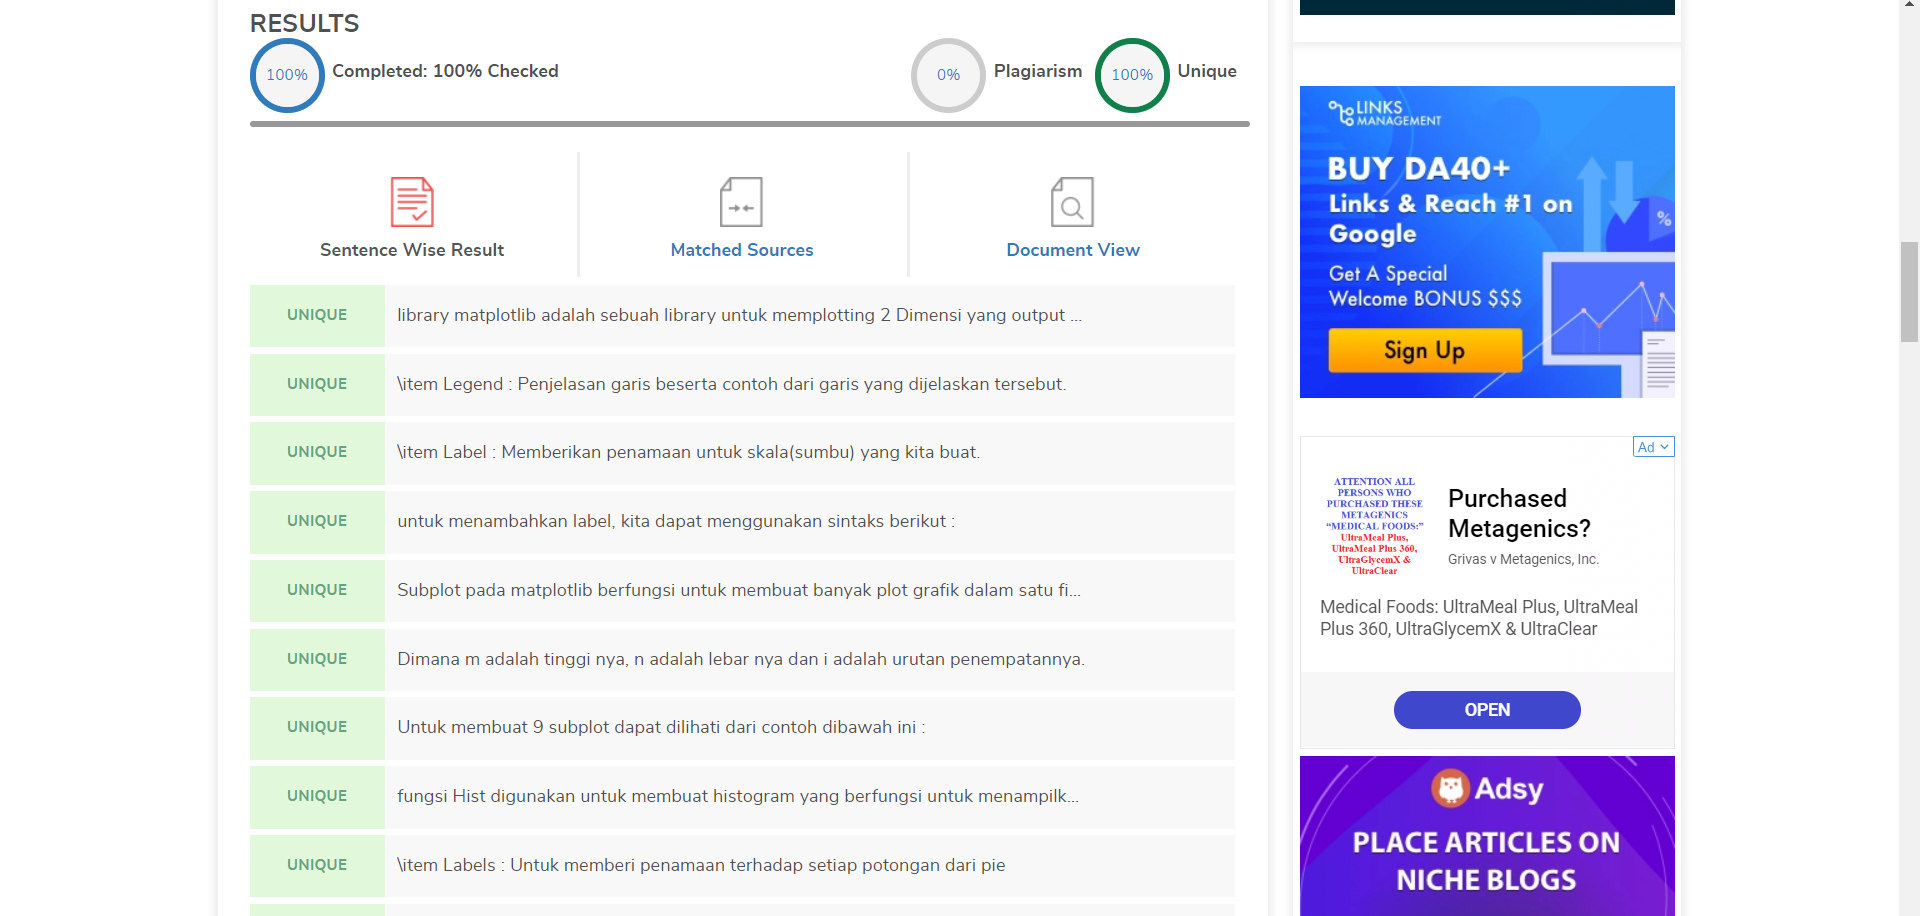
\includegraphics[width=0.5\textwidth]{figures/6/1174040/Teori/1174040_plagiat.png}}
            \caption{Cek Plagiarisme}
            \label{1174040_chap6_plagiat}
            \end{figure}
			
\section{Irvan Rizkiansyah/1174043}
	\subsection{Nomor 1}
		matplotlib merupakan library plotting 2D Python dan berfungsi untuk membuat plot, histogram, grafik batang, scatterplot, dan masih banyak yang lainnya hanya dengan beberapa baris code saja.
		
	\subsection{Nomor 2}
	Pembuatan sumbu X dan Y di matplotlib, mirip dengan membuat sebuah variabel yang mempunyai array. Kemudian variabel yang dibuat yang nanti-nya akan menjadi sumbu X dan Y dan akan dipanggil menggunakan fungsi plot.
		\lstinputlisting[firstline=8, lastline=14]{src/6/1174043/Teori/chap6_1174043_no2.py}
	
	\subsection{Nomor 3}
	Perbedaan fungsi yang ada pada matplotlib :
		\begin{itemize}
			\item Fungsi scatter atau plot sebaran merupakan sebuah grafik yang menunjukkan hubungan dari dua set data, seperti halnya hubungan dari tinggi badan dan berat badan.
			Cara menggunakannya dengan memanggil fungsi scatter yang terdapat pada matplotlib \begin{verbatim} matplotlib.pyplot.scatter(x,y) \end{verbatim}
			
			\item Fungsi histogram merupakan sebuah grafik yang akan menampilkan frekuensi data menggunakan sebuah batang.
			Cara menggunakannya dengan memanggil fungsi hist yang terdapat pada matplotlb \begin{verbatim} matplotlib.pyplot.hist(x,y) \end{verbatim}
			
			\item Fungsi plot garis atau plot sinus merupakan sebuah grafik yang menunjukkan frekuensi data menggunakan garis.
			Cara menggunakannya dengan memanggil fungsi plot yang terdapat pada matplotlib \begin{verbatim} matplotlib.pyplot.plot(x,y) \end{verbatim}
			
		\end{itemize}
	Dan masih banyak yang lainnya.
	\subsection{Nomor 4}
	Fungsi legend merupakan dimana akan menamai sebuah bar pada grafik untuk membedakan bar tersebut dengan bar yang lainnya, dimana jika terdapat banyak bar pada grafik tersebut. Sedangkan fungsi label untuk menamai sumbu x dan sumbu y.
	Cara menggunakannya hanya tinggal memanggil fungsi legend dan fungsi label yang terdapat pada matplotlib dan memberikan nama untuk legend dan label tersebut. Contohnya :
		\lstinputlisting[firstline=8, lastline=19]{src/6/1174043/Teori/chap6_1174043_legend.py}
	
	\subsection{Nomor 5}
	Fungsi subplot adalah untuk memanggil banyak grafik hanyak dengan sekali panggil saja. Cara kerja dari fungsi subplot ini sendiri cukup simpel, dimana cukup memanggil fungsi subplot yang terdapat pada matplotlib 
	\begin{verbatim} matplotlib.pyplot.subplot(nbaris, nkolom, index) \end{verbatim}
	Dibawah ini merupakan ilustrasi dan parameter apa saja yang digunakan jika ingin menggambar plot dengan 9 sub plot :
		\lstinputlisting[firstline=8, lastline=54]{src/6/1174043/Teori/chap6_1174043_subplot.py}
		
	\subsection{Nomor 6}
	Matplotlib mengenal beberapa format untuk color diantaranya :
		\begin{itemize}
			\item RGB atau RGBA contohnya (0.1, 0.2, 0.5)
			\item hex RGB atau RGBA contohnya '\#0F0F0F
			\item Representasi string dari nilai float contohnya '0.5'
			\item atau hanya seperti kata awal dari warna tersebut yang ingin digunakan contohnya warna Cyan maka hanya perlu menggunakan 'c', warna Green maka hanya perlu menggunakan 'g' dan masih banyak yang lainnya seperti 'b', 'r', 'm', dan yang lainnya
			\item X11/CSS4 nama warna
			\item nama dari xkcd color survey contohnya 'xkcd:sky blue'
			\item Tableau Color dari 'T10' pallette kategorikal contohnya 'tab:olive'
			
		\end{itemize}
	
	\subsection{Nomor 7}
	Fungsi hist merupakan fungsi untuk menggunakan grafik bar atau batang, dimana frekuensi setiap elemen data yang ada pada daftar ditunjukkan dengan grafik histogram. Angka yang dikelompokkan dalam bentuk rentang tertentu yang sudah di tentukan dsebut bins.
		\lstinputlisting[firstline=8, lastline=12]{src/6/1174043/Teori/chap6_1174043_histogram.py}
	
	\subsection{Nomor 8}
	Parameter yang terdapat pada fungsi pie :
		\begin{itemize}
			\item labels : dimana berfungsi untuk memberi nama untuk setiap slice yang terdapat pada grafik pie
			\item colors : dimana berfungsi untuk memberikan warna untuk setiap slice yang terdapat pada gradik pie
			\item startangle : dimana berfungsi jika tidak tidak ada, maka awalan putaran dari grafik pie berlawanan dari arah jarum jam dari titik sumbu x
			\item shadow : dimana berfungsi untuk memberikan efek grafis bayangan pada grafik pie
			\item explode : dimana berfungsi untuk menentukan fraksi dari jari-jari untuk mengimbangi setiap slice menggunakan sumbu x
			\item autopct : string atau fungsi yang digunakan untuk label pada slice dengan nilai numerik, maka label akan ditempatkan didalam slice.			
		\end{itemize}

\section{Luthfi Muhammad Nabil/1174035}
\subsection{Soal 1}
Apa itu fungsi library matplotlib

Library matplotlib adalah library bahasa pemrograman python untuk menampilkan grafik - grafik sehingga data dapat divisualisasikan dengan lebih baik. Isi dari grafik tersebut dapat menggunakan data sesuai kebutuhan. Matplotlib sudah digunakan banyak aplikasi data sains untuk menampilkan visualisasi data yang berupa grafik. 

\subsection{Soal 2}
Jelaskan langkah-langkah membuat sumbu X dan Y di matplotlib

Pada library matplotlib, hanya membutuhkan dua variabel atau dua kumpulan data yang memiliki posisi sama. Isi dari data tersebut menggunakan nilai angka dan isinya dapat berupa integer atau float. Berikut contoh dari koding menampilkan data dengan sumbu X dan Y : 
\lstinputlisting[firstline=2, lastline=6]{src/6/1174035/Teori/chap6_1174035_Teori.py}
Berikut hasilnya terdapat pada gambar \ref{Contoh_Soal2}
\begin{figure} [ht]
	\centerline{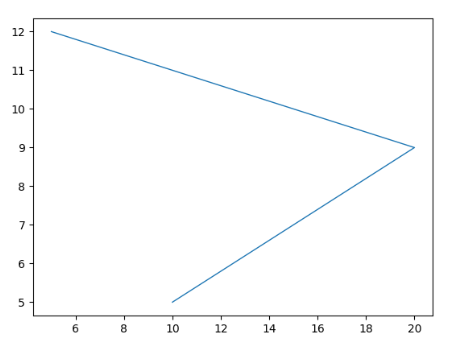
\includegraphics[width=0.6\textwidth]{figures/6/1174035/Teori/Soal2.png}}
	\caption{Contoh Pengaplikasian Sumbu X dan Y}
	\label{Contoh_Soal2}
\end{figure}

\subsection{Soal 3}
Jelaskan bagaimana perbedaan fungsi dan cara pakai untuk berbagai jenis plot di matplotlib
\begin{itemize}
	\item Grafik Garis
	
	Untuk plot pada diagram garis, dibutuhkan data nilai angka yang dapat berupa satu atau dua kumpulan data. Berikut pengaplikasian untuk diagram garis : 
	\lstinputlisting[firstline=9, lastline=12]{src/6/1174035/Teori/chap6_1174035_Teori.py}
	Atau dapat juga mengubah jalur garis dengan 2 kumpulan angka seperti berikut : 
	\lstinputlisting[firstline=15, lastline=18]{src/6/1174035/Teori/chap6_1174035_Teori.py}
	\begin{figure} [ht]
		\centerline{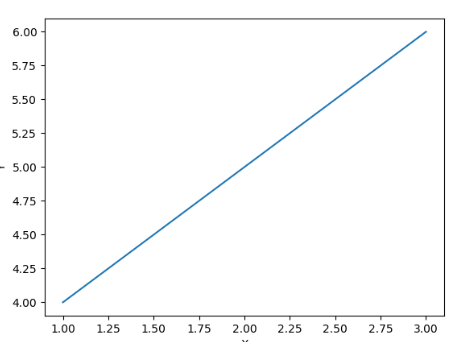
\includegraphics[width=0.6\textwidth]{figures/6/1174035/Teori/Soal3Garis.png}}
		\caption{Contoh Grafik Garis}
		\label{Contoh_Soal3Garis}
	\end{figure}
	
	\item Grafik Titik
	
	Untuk plot pada diagram titik, dapat melakukan langkah seperti berikut : 
	\lstinputlisting[firstline=21, lastline=26]{src/6/1174035/Teori/chap6_1174035_Teori.py}
	Terlihat perbedaannya pada penambahan parameter ketiga dengan isinya yaitu 'ro'
	\begin{figure} [ht]
		\centerline{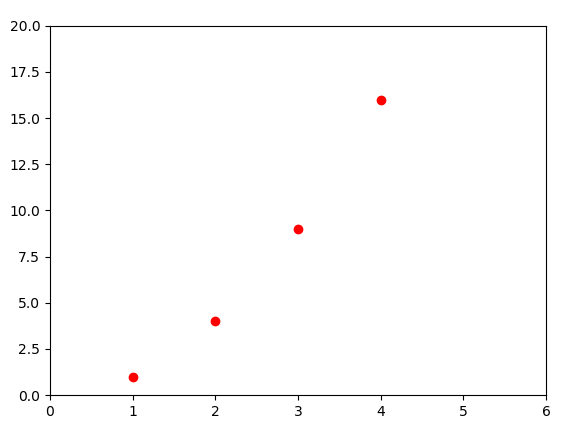
\includegraphics[width=0.6\textwidth]{figures/6/1174035/Teori/Soal3Titik.png}}
		\caption{Contoh Grafik Titik}
		\label{Contoh_Soal3Titik}
	\end{figure}
	
	\item Grafik Batang
	
	Untuk plot diagram batang diperlukan koding baru menggunakan plt.bar(). Contoh pengaplikasian dapat diaplikasikan sebagai berikut : 
	\lstinputlisting[firstline=29, lastline=31]{src/6/1174035/Teori/chap6_1174035_Teori.py}
	Hasil dapat dilihat pada gambar \ref{Contoh_Soal3Batang}
	\begin{figure} [ht]
		\centerline{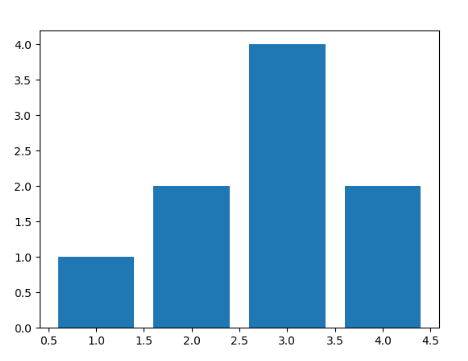
\includegraphics[width=0.6\textwidth]{figures/6/1174035/Teori/Soal3Batang.png}}
		\caption{Contoh Grafik Batang}
		\label{Contoh_Soal3Batang}
	\end{figure}
	
	\item Grafik Lingkaran
	
	Untuk plot diagram batang perlu menggunakan subplot. Berikut contoh pengaplikasiannya : 
	\lstinputlisting[firstline=34, lastline=43]{src/6/1174035/Teori/chap6_1174035_Teori.py}
	Hasil dapat dilihat pada gambar \ref{Contoh_Soal3Pie}
	\begin{figure} [ht]
		\centerline{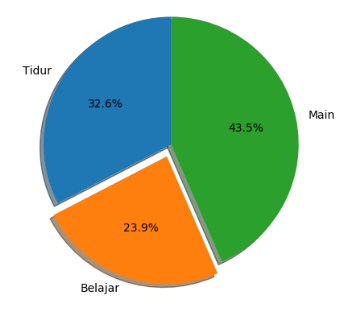
\includegraphics[width=0.6\textwidth]{figures/6/1174035/Teori/Soal3Pie.png}}
		\caption{Contoh Grafik Pie}
		\label{Contoh_Soal3Pie}
	\end{figure}
\end{itemize}

\subsection{Soal 4}
Jelaskan bagaimana cara menggunakan legend dan label serta kaitannya dengan fungsi tersebut
\begin{itemize}
\item Label

Untuk menggunakan label, hanya perlu menambahkan sintaks plt.xlabel() atau plt.ylabel(). Label berfungsi untuk memberikan label pada setiap garis atau label untuk gambar yang ada. Berikut contoh untuk menambahkan label pada matplotlib : 
\lstinputlisting[firstline=46, lastline=52]{src/6/1174035/Teori/chap6_1174035_Teori.py}
Pada sintaks berikut, akan menambahkan label pada sumbu x dengan tulisan 'X', begitu juga dengan sumbu y dengan label 'Y'. Berikut hasilnya pada gambar \ref{Contoh_Soal4Label} 
\begin{figure} [ht]
	\centerline{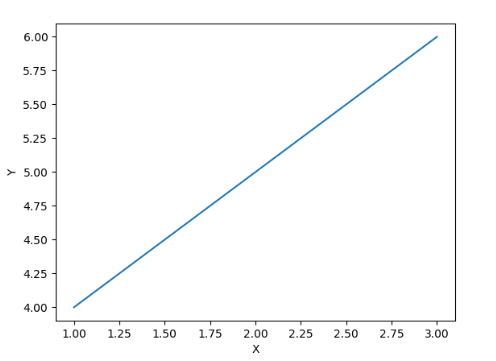
\includegraphics[width=0.6\textwidth]{figures/6/1174035/Teori/Soal4Label.png}}
	\caption{Contoh Pengaplikasian Label}
	\label{Contoh_Soal4Label}
\end{figure}

\item Legend

Untuk menggunakan legend, perlu mengadakan label saat menginisiasi sebuah plot. Berikut contoh penggunaan legend : 
\lstinputlisting[firstline=54, lastline=59]{src/6/1174035/Teori/chap6_1174035_Teori.py}

Pada sintaks plt.plot(), terdapat parameter untuk menginput label yang isinya 'Garis Satu' untuk mengatur isi atau judul dari label tersebut. Lalu plt.legend() adalah sintaks untuk menunjukan legend yang akan dimunculkan. Berikut contoh dari pengaplikasiannya pada gambar \ref{Contoh_Soal4Legend} 
\begin{figure} [ht]
	\centerline{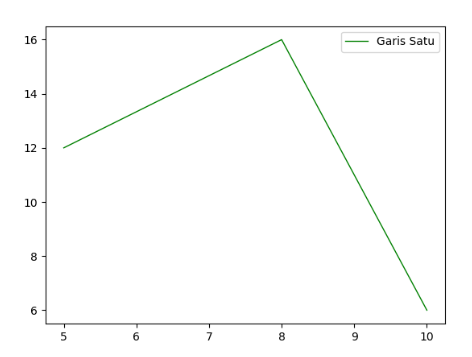
\includegraphics[width=0.6\textwidth]{figures/6/1174035/Teori/Soal4Legend.png}}
	\caption{Contoh Pengaplikasian Legend}
	\label{Contoh_Soal4Legend}
\end{figure}
\end{itemize}

\subsection{Soal 5}
Jelaskan apa fungsi dari subplot di matplotlib, dan bagaimana cara kerja dari fungsi subplot

Subplot adalah fungsi untuk menampilkan beberapa diagram pada satu aplikasi atua sintaks. Untuk menginisiasi subplot, dapat menggunakan fungsi plt.subplot() dan memasukan ukuran subplot di dalamnya (Contoh : plt.subplot(331)). Pada fungsi plt.subplot(331), angka pertama pada contoh merupakan jumlah baris yang dapat dipakai dan angka kedua merupakan jumlah kolom yang dapat dipakai sedangkan angka ketiga merupakan di baris dan kolom berapa grafik akan disimpan. Posisi grafik dimulai dari kiri atas dan berpindah ke kanan dan jika sudah mencapai batas kolom maka akan berpindah ke baris selanjutnya yang dimulai dari kiri kembali. Contoh penggunaan subplot : 
\lstinputlisting[firstline=61, lastline=103]{src/6/1174035/Teori/chap6_1174035_Teori.py}
Berikut hasil yang didapat pada koding berikut ditampilkan pada gambar \ref{Contoh_Soal5}
\begin{figure} [ht]
	\centerline{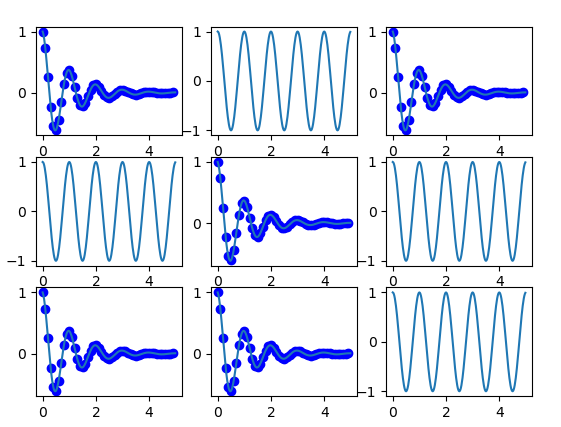
\includegraphics[width=0.6\textwidth]{figures/6/1174035/Teori/Soal5.png}}
	\caption{Contoh Pengaplikasian Subplot}
	\label{Contoh_Soal5}
\end{figure}

\subsection{Soal 6}
Sebutkan semua parameter color yang bisa digunakan

\begin{itemize}
	\item b : Untuk memberikan warna biru
	\item g : Untuk memberikan warna hijau
	\item r : Untuk memberikan warna merah
	\item c : Untuk memberikan warna biru muda
	\item m : Untuk memberikan warna pink
	\item y : Untuk memberikan warna kuning
	\item k : Untuk memberikan warna hitam
	\item w : Untuk memberikan warna putih
\end{itemize}

\subsection{Soal 7}
Jelaskan bagaimana cara kerja dari fungsi hist

Fungsi hist pada library matplotlib yaitu menhistorgramkan kumpulan data yang akan ditampilkan biasanya berupa grafik batang. Grafik akan dimasukkan beberapa data dan diambil frekuensi dari data tersebut. Berikut contoh koding dari histogram : 
\lstinputlisting[firstline=106, lastline=113]{src/6/1174035/Teori/chap6_1174035_Teori.py}
Berikut hasil dari histogram yang ada pada gambar \ref{Contoh_Soal7}
\begin{figure} [ht]
	\centerline{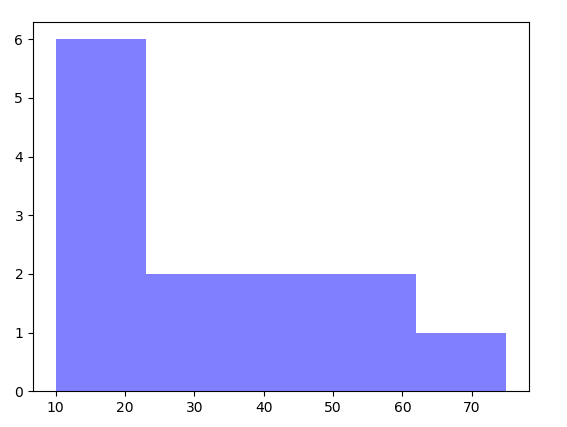
\includegraphics[width=0.6\textwidth]{figures/6/1174035/Teori/Soal7.png}}
	\caption{Contoh Pengaplikasian Histogram}
	\label{Contoh_Soal7}
\end{figure}
\subsection{Soal 8}
Jelaskan lebih mendalam tentang parameter dari fungsi pie.

\begin{itemize}
	\item labels : Isi dengan tipe data list dan tidak wajib untuk digunakan. Fungsi parameter labels untuk memberi label pada setiap pecahan data yang ada pada grafik pie yang ditampilkan.
	\item colors : Tipe data array atau sejenis dan tidak wajib untuk digunakan. Fungsi parameter colors untuk mengganti warna pada setiap pecahan yang ada. Jika tidak digunakan atau ditentukan, maka warna yang akan dipakai adalah warna yang aktif atau standar.
	\item startangle : Tipe data pecahan atau float, tidak wajib untuk digunakan. Fungsi parameter startangle adalah fungsi untuk memutar grafik agar berubah posisi dengan acuan yaitu angle awalan dari grafik pie.
	\item shadow : Bertipe data boolean dan tidak wajib digunakan. Fungsi parameter shadow digunakan untuk membuat bayangan pada bawah grafik pie yang ditampilkan. 
	\item explode : Bertipe data array atau sejenis dan tidak wajib digunakan. Fungsi parameter explode adalah menentukan radius untuk mengimbangi setiap pecahan pada grafik pie. Jika radius lebih dari 0 maka pecahan akan mulai menjauh dari pusat dan terlihat seperti keluar dari grafik lingkaran tersebut.
	\item autopct : Bertipe data string atau fungsi dan tidak wajib digunakan. Fungsi parameter autopct adalah memberi label pada irisan dengan labelnya berupa fungsi atau string. 
\end{itemize}

\subsection{Plagiarisme}
Berikut hasil pengecekan plagiarisme untuk bagian teori terdapat pada gambar \ref{Plagiarisme}.
\begin{figure} [ht]
	\centerline{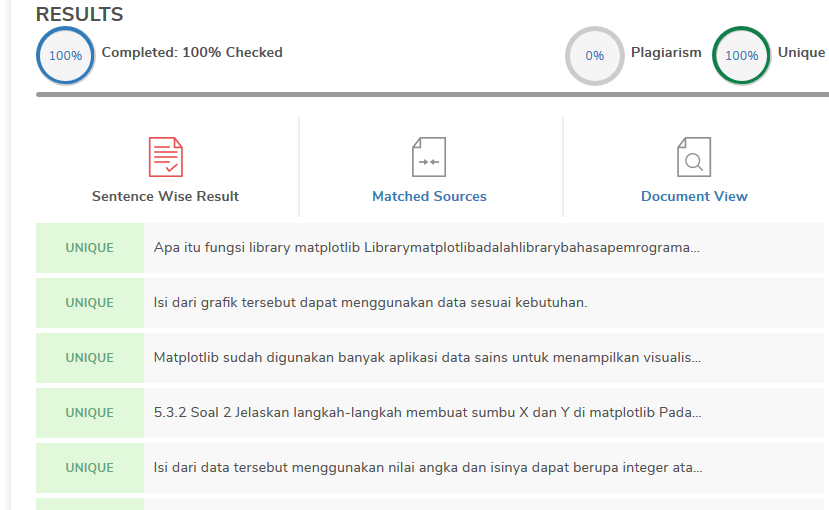
\includegraphics[width=0.6\textwidth]{figures/6/1174035/Teori/Plagiarisme.png}}
	\caption{Cek Plagiarisme}
	\label{Plagiarisme}
\end{figure}


\section{Faisal Najib Abdullah 1174042}
\subsection{Teori}
\subsubsection{Soal No. 1}
\hfill \break
Apa itu fungsi library matplotlib?

\hfill \break
Matplotlib merupakan salah satu library Python 2D yang dapat menghasilkan plot dengan kualitas yang tinggi dalam berbagai format dan dapat digunakan di berbagai platform. Matplotlib berfungsi sebagai pembuat grafik di berbagai platform, seperti Python dan Jupyter. Grafik yang dibuat menggunakan Matplotlib bisa dibuat dalam berbagai bentuk, seperti grafik garis, batang, lingkaran, histogram, dan sebagainya.

\subsubsection{Soal No. 2}
\hfill \break
Jelaskan langkah-langkah membuat sumbu X dan Y di matplotlib!

\begin{enumerate}
	\item Pertama import library Matplotlib.	
	\lstinputlisting[firstline=2, lastline=2]{src/6/1174042/1174042.py}
	
	\item Buat variabel x yang menampung list untuk sumbu x dan variabel y yang menampung list untuk sumbu y.	
	\lstinputlisting[firstline=4, lastline=5]{src/6/1174042/1174042.py}
	
	\item Panggil fungsi plot dan isi parameter pertama dengan variabel x dan parameter kedua dengan variabel y.
	\lstinputlisting[firstline=7, lastline=7]{src/6/1174042/1174042.py}	

	\item Lalu panggil plot tadi dengan memanggil fungsi show.
	\lstinputlisting[firstline=9, lastline=9]{src/6/1174042/1174042.py}
	
\end{enumerate}
\hfill \break
\textbf{Kode Program}

\lstinputlisting[caption = Kode program membuat diagram menggunakan Matplotlib., firstline=2, lastline=9]{src/6/1174042/1174042.py}

\hfill \break
\textbf{Hasil Compile}

\begin{figure}[H]
	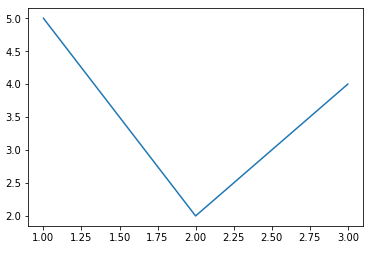
\includegraphics[width=12cm]{figures/6/1174042/1.png}
	\centering
	\caption{Hasil compile membuat diagram menggunakan Matplotlib.}
\end{figure}
 
\subsubsection{Soal No. 3}
\hfill \break
Jelaskan bagaimana perbedaan fungsi dan cara pakai untuk berbagai jenis(bar, histogram ,scatter ,line, dll) jenis plot di matplotlib!

\begin{enumerate}
	\item \textbf{Bar Graph}
	
	Perbedaan bar graph dengan jenis plot yang lain adalah bar graph menggunakan bar atau batang-batang untuk membandingkan data di antara berbagai kategori.
	
	\textbf{Kode Program}
	
	\lstinputlisting[caption = Kode program membuat bar graph menggunakan Matplotlib., firstline=13, lastline=25]{src/6/1174042/1174042.py}
	
	\textbf{Hasil Compile}
	
	\begin{figure}[H]
		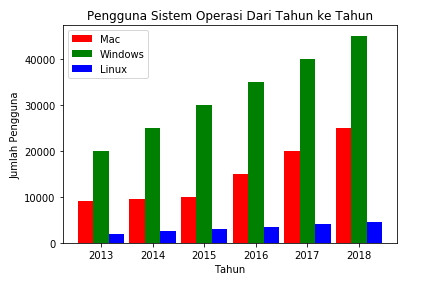
\includegraphics[width=12cm]{figures/6/1174042/2.png}
		\centering
		\caption{Hasil compile membuat bar graph menggunakan Matplotlib.}
	\end{figure}
	
	\item \textbf{Histogram}
	
	Perbedaan histogram dengan jenis plot yang lain adalah histogram akan membuat plot dimana plot yang dimunculkan merupakan gabungan dari beberapa data yang telah dikelompokkan.
	
	\textbf{Kode Program}
	
	\lstinputlisting[caption = Kode program membuat histogram menggunakan Matplotlib., firstline=29, lastline=36]{src/6/1174042/1174042.py}
	
	\textbf{Hasil Compile}
	
	\begin{figure}[H]
		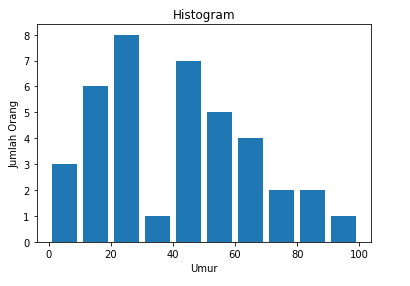
\includegraphics[width=12cm]{figures/6/1174042/3.png}
		\centering
		\caption{Hasil compile membuat histogram menggunakan Matplotlib.}
	\end{figure}
	
	\item \textbf{Scatter Plot}
	
	Perbedaan scatter plot dengan jenis plot lain adalah scatter plot menampilkan data sebagai kumpulan titik, masing-masing memiliki nilai satu variabel yang menentukan posisi pada sumbu horizontal dan nilai variabel lain menentukan posisi pada sumbu vertikal.
	
	\textbf{Kode Program}
	
	\lstinputlisting[caption = Kode program membuat scatter plot menggunakan Matplotlib., firstline=40, lastline=53]{src/6/1174042/1174042.py}
	
	\textbf{Hasil Compile}
	
	\begin{figure}[H]
		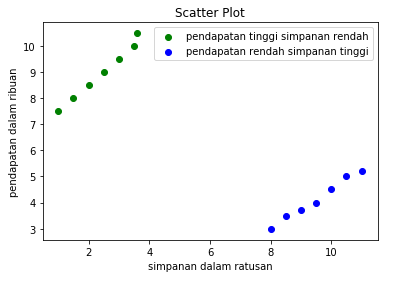
\includegraphics[width=12cm]{figures/6/1174042/4.png}
		\centering
		\caption{Hasil compile membuat scatter plot menggunakan Matplotlib.}
	\end{figure}
	
	\item \textbf{Area Plot}
	
	Perbedaan area plot dengan jenis plot lain adalah area plot digunakan untuk melacak perubahan dari waktu ke waktu untuk dua atau lebih kelompok terkait yang membentuk satu kategori secara keseluruhan.
	
	\textbf{Kode Program}
	
	\lstinputlisting[caption = Kode program membuat diagram menggunakan Matplotlib., firstline=57, lastline=76]{src/6/1174042/1174042.py}
	
	\textbf{Hasil Compile}
	
	\begin{figure}[H]
		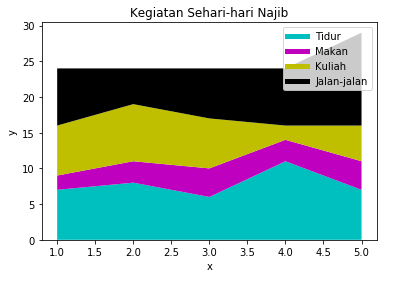
\includegraphics[width=12cm]{figures/6/1174042/5.png}
		\centering
		\caption{Hasil compile membuat diagram menggunakan Matplotlib.}
	\end{figure}
	
	\item \textbf{Pie Plot}
	
	Perbedaan pie plot dengan jenis plot lain adalah pie plot digunakan untuk menunjukkan persentase atau data proporsional di mana setiap potongan pie mewakili kategori.
	
	\textbf{Kode Program}
	
	\lstinputlisting[caption = Kode program membuat Pie Plot menggunakan Matplotlib., firstline=86, lastline=101]{src/6/1174042/1174042.py}
	
	\textbf{Hasil Compile}
	
	\begin{figure}[H]
		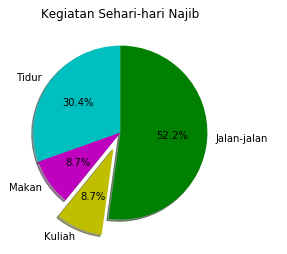
\includegraphics[width=9cm]{figures/6/1174042/6.png}
		\centering
		\caption{Hasil compile membuat Pie Plot menggunakan Matplotlib.}
	\end{figure}
	
	\item \textbf{Line Graph}
	
	Perbedaan line graph dengan jenis plot lain adalah line graph menampilkan diagram dalam bentuk garis.
	
	\textbf{Kode Program}
	
	\lstinputlisting[caption = Kode program membuat diagram menggunakan Matplotlib., firstline=105, lastline=113]{src/6/1174042/1174042.py}
	
	\textbf{Hasil Compile}
	
	\begin{figure}[H]
		\includegraphics[width=12cm]{figures/6/1174042/7.png}
		\centering
		\caption{Hasil compile membuat diagram menggunakan Matplotlib.}
	\end{figure}
	
\end{enumerate}

\subsubsection{Soal No. 4}
\hfill \break
Jelaskan bagaimana cara menggunakan legend dan label serta kaitannya dengan fungsi tersebut!

\begin{enumerate}
	\item Untuk menggunakan legend definisikan parameter label di tiap fungsi plot. Parameter label digunakan untuk memberikan label pada line sebagai pembeda antar line.
	
	\lstinputlisting[caption = Kode program menggunakan parameter label dengan Matplotlib., firstline=123, lastline=124]{src/6/1174042/1174042.py}
	
	\item Kemudian panggil fungsi legend.
	
	\lstinputlisting[caption = Kode program memanggil fungsi legend dengan Matplotlib., firstline=128, lastline=128]{src/6/1174042/1174042.py}
\end{enumerate}

\hfill \break
\textbf{Kode Program}

\lstinputlisting[caption = Kode program membuat diagram menggunakan Matplotlib., firstline=117, lastline=130]{src/6/1174042/1174042.py}

\hfill \break
\textbf{Hasil Compile}

\begin{figure}[H]
	\includegraphics[width=12cm]{figures/6/1174042/8.png}
	\centering
	\caption{Hasil compile membuat diagram menggunakan Matplotlib.}
\end{figure}

\subsubsection{Soal No. 5}
\hfill \break
Jelaskan apa fungsi dari subplot di matplotlib, dan bagaimana cara kerja dari fungsi subplot, sertakan ilustrasi dan gambar sendiri dan apa parameternya jika ingin menggambar plot dengan 9 subplot di dalamnya!

\hfill \break
Fungsi subplot adalah untuk membuat beberapa plot di dalam satu gambar.
\hfill \break
Cara kerja subplot, yaitu fungsi subplot memiliki parameter pertama adalah jumlah kolom, parameter kedua adalah jumlah baris, dan parameter ketiga adalah index plot keberapanya.

\hfill \break
\textbf{Kode Program}

\lstinputlisting[caption = Kode program membuat subplot menggunakan Matplotlib., firstline=134, lastline=146]{src/6/1174042/1174042.py}

\hfill \break
\textbf{Hasil Compile}

\begin{figure}[H]
	\includegraphics[width=12cm]{figures/6/1174042/9.png}
	\centering
	\caption{Hasil compile membuat subplot menggunakan Matplotlib.}
\end{figure}

\subsubsection{Soal No. 6}
\hfill \break
Sebutkan semua parameter color yang bisa digunakan (contoh:  m,c,r,k,...  dkk)!

\begin{itemize}
	\item 'b' (blue)
	\item 'g' (green)
	\item 'r' (red)
	\item 'c' (cyan)
	\item 'm' (magenta)
	\item 'y' (yellow)
	\item 'k' (black)
	\item 'w' (white)
\end{itemize}

\subsubsection{Soal No. 7}
\hfill \break
Jelaskan bagaimana cara kerja dari fungsi hist, sertakan ilustrasi dan gambar sendiri!

\hfill \break
Cara kerja dari fungsi hist yaitu fungsi hist akan menerima parameter yang diberikan, kemudian fungsi hist akan dieksekusi sesuai dengan parameter yang diberikan.

\hfill \break
\textbf{Kode Program}

\lstinputlisting[caption = Kode program membuat diagram menggunakan Matplotlib., firstline=150, lastline=157]{src/6/1174042/1174042.py}

\hfill \break
\textbf{Hasil Compile}

\begin{figure}[H]
	\includegraphics[width=12cm]{figures/6/1174042/10.png}
	\centering
	\caption{Hasil compile membuat diagram menggunakan Matplotlib.}
\end{figure}

\subsubsection{Soal No. 8}
\hfill \break
 Jelaskan lebih mendalam tentang parameter dari fungsi pie diantaranya labels, colors, startangle, shadow, explode, autopct!
 
 \begin{itemize}
 	\item labels : untuk memberikan label di tiap persentase.
 	\item colors : untuk memberikan warna di tiap persentase.
 	\item startangle : untuk memutar plot sesuai dengan derajat yang ditentukan.
 	\item shadow : untuk memberikan bayangan pada plot.
 	\item explode : untuk memisahkan antar tiap potongan pie pada plot.
 	\item autopct : untuk menentukan jumlah angka dibelakang koma.
 \end{itemize}

\subsection{Plagiarisme}
Berikut hasil pengecekan plagiarisme untuk bagian teori.
\begin{figure}[H]
	\includegraphics[width=12cm]{figures/6/1174042/plagiat.png}
	\centering
	\caption{Plagiarisme}
\end{figure}

\section{Dika Sukma Pradana 1174050}
\subsection{Pemahaman Teori}
\begin{enumerate}
\item Apa itu fungsi library matplotlib?
\par
Matplotlib adalah perpustakaan merencanakan untuk bahasa pemrograman Python dan ekstensi numerik matematika NumPy. Ini menyediakan API berorientasi objek untuk menanamkan plot ke aplikasi menggunakan toolkit GUI untuk tujuan umum seperti Tkinter, wxPython, Qt, atau GTK +. Ada juga antarmuka "pylab" prosedural yang didasarkan pada mesin negara (seperti OpenGL), yang dirancang agar mirip dengan MATLAB, meskipun penggunaannya tidak disarankan. PiPy menggunakan Matplotlib.
\par
Matplotlib awalnya ditulis oleh John D. Hunter, memiliki komunitas pengembangan aktif, dan didistribusikan di bawah lisensi gaya BSD. Michael Droettboom dinominasikan sebagai pengembang utama matplotlib sesaat sebelum kematian John Hunter pada Agustus 2012, dan selanjutnya bergabung dengan Thomas Caswell.
\par
Pada 23 Juni 2017, matplotlib 2.0.x mendukung versi Python 2.7 hingga 3.6. Matplotlib 1.2 adalah versi pertama dari matplotlib untuk mendukung Python 3.x. Matplotlib 1.4 adalah versi terakhir dari Matplotlib untuk mendukung Python 2.6.
\par
Matplotlib telah berjanji untuk tidak mendukung Python 2 hingga 2020 dengan menandatangani Pernyataan Python 3

\item Jelaskan langkah-langkah membuat sumbu X dan Y di matplotlib!
Pada Matplotlib untuk membuat sumbu X dan Y dapat dilakukan dengan cara yaitu :
\lstinputlisting[firstline=1, lastline=7]{src/6/1174050/Teori/no2.py}

\item Jelaskan bagaimana perbedaan fungsi dan cara pakai untuk berbagai jenis(bar,histogram,scattdll) jenis plot di matplotlib!
\begin{itemize}
\item Sebuah plot sebaran/titik adalah sebuah grafik yang menunjukkan hubungan antara dua set data.
\lstinputlisting[firstline=1, lastline=6]{src/6/1174050/Teori/scatter.py}
\begin{figure}[H]
\centering
\includegraphics[width=7cm]{figures/6/1174050/Teori/3scatter.png}
\caption{Scatter}
\end{figure}

\item Sebuah histogram adalah grafik yang menampilkan frekuensi data menggunakan batang, dimana angka dikelompokkan dalam rentang tertentu. Dengan kata lain, frekuensi setiap elemen data di dalam daftar ditunjukkan menggunakan histogram. Angka yang dikelompokkan dalam bentuk rentang tertentu disebut bins.
\lstinputlisting[firstline=1, lastline=6]{src/6/1174050/Teori/histo.py}
\begin{figure}[H]
\centering
\includegraphics[width=7cm]{figures/6/1174050/Teori/3histo.png}
\caption{Histogram}
\end{figure}


\item pie chart adalah diagram yang digunakan untuk membandingkan antar bagian terhadap total. biasanya pie chart dalam bentuk persentase karena nilainya merupakan bagian-bagian yang dijumlah menjadi satu. sehingga bisa lihat kontribusi paling besar atau paling kecil dalam membentuk nilai. Pie chart digunakan untuk perbandingan yang sedikit. pie chart digunakan untuk membandingkan antar bagian terhadap total.
\lstinputlisting[firstline=1, lastline=23]{src/6/1174050/Teori/pie.py}
\begin{figure}[H]
\centering
\includegraphics[width=7cm]{figures/6/1174050/Teori/3pie.png}
\caption{pie chart}
\end{figure}

\item Bagan area benar-benar mirip dengan bagan garis, kecuali area antara sumbu x dan garis diisi dengan warna atau bayangan. Ini mewakili evolusi variabel numerik mengikuti variabel numerik lainnya. Jika kamu ingin mewakili evolusi ini untuk beberapa grup dalam waktu yang bersamaan, Anda mungkin tertarik dengan bagan area bertumpuk, di mana setiap grup ditampilkan satu sama lain.
\lstinputlisting[firstline=1, lastline=21]{src/6/1174050/Teori/area.py}
\begin{figure}[H]
\centering
\includegraphics[width=7cm]{figures/6/1174050//Teori/area.png}
\caption{bagan area}
\end{figure}

\end{itemize}

\item Jelaskan bagaimana cara menggunakan legend dan label serta kaitannya dengan
fungsi tersebut!
\par
Legenda adalah penjelasan garis dilengkapi dengan sampel garis yang dijelaskan. Untuk membuat legenda pada plot anda dapat menggunakan syntax fungsi legend yang dapat dituliskan sebagai berikut:
\lstinputlisting[firstline=69, lastline=69]{src/6/1174050/Teori/6.py}
\begin{figure}[H]
\centering
\includegraphics[width=4cm]{figures/6/1174050/Teori/legen.png}
\caption{legend}
\end{figure}
\par
Untuk menambah label pada garis sumbu pada grafik dapat menggunakan syntax fungsi xlabel dan fungsi ylabel pada MATLAB. Kedua label ditulis setelah syntax deklarasi plot.
\lstinputlisting[firstline=40, lastline=40]{src/6/1174050/Teori/6.py}
\begin{figure}[H]
\centering
\includegraphics[width=4cm]{figures/6/1174050/Teori/label.png}
\caption{label}
\end{figure}


\item Jelaskan apa fungsi dari subplot di matplotlib, dan bagaimana cara kerja dari
fungsi subplot, sertakan ilustrasi dan gambar sendiri dan apa parameternya jika
ingin menggambar plot dengan 9 subplot di dalamnya
\par
Pada saat fungsi plot dijalankan, grafik atau gelombang akan ditampilkan dalam figure yang aktif. Untuk beberapa kasus, perlu menampilkan plot grafik atau gelombang dalam figure atau gambar yang berbeda maupun menampilkan lebih dari satu plot dalam satu gambar. Hal ini bisa terjadi jika menggbungkan beberapa plot dalam 1 figure.
\lstinputlisting[firstline=72, lastline=104]{src/6/1174050/Teori/6.py}
\begin{figure}[H]
\centering
\includegraphics[width=7cm]{figures/6/1174050/Teori/subplot.png}
\caption{Subplot}
\end{figure}


\item Sebutkan semua parameter color yang bisa digunakan!
\par
Kode warna yang digunakan dalam python adalah sebagai berikut:
R adalah warna Merah
G adalah warna Hijau
B adalah warna Biru
M adalah warna Ungu
Y adalah warna Kuning
C adalah warna Biru Muda
K adalah warna Hitam

\item Jelaskan bagaimana cara kerja dari fungsi hist, sertakan ilustrasi dan gambar
sendiri!
\par
pada fungsi histogram titik koordinat tidak boleh sama karena dalam diagram ini digunakan untuk mendata selisih dari hasil rentang nilai tertentu.

\begin{figure}[H]
\centering
\includegraphics[width=7cm]{figures/6/1174050/Teori/3histo.png}
\caption{Histogram}
\end{figure}


\item Jelaskan lebih mendalam tentang parameter dari fungsi pie diantaranya labels,
colors, startangle, shadow, explode, autopct
\begin{itemize}
\item labels digunakan untuk memberi label/penjelasan dari bagian pie chart yang kita buat.
\item colors digunakan untuk mewarnai pie chart diagram yang telah dibuat, membuat warna yang berbeda antar bagian.
\item startangle digunakan untuk membuat diagram/chart mem-flip atau berbalik arah.
\item explode digunakan untuk menonjolkan salah satu bagian dari pie chart.
\item shadows digunakan untuk memberi bayangan pada pie chart yang kita buat.
\item autopct digunakan untuk memberi persen dari bagian-bagian pie chart yang kita buat.
\end{itemize}

\item Bebas Plagiarisme
\begin{figure}[H]
\centering
\includegraphics[width=7cm]{figures/6/1174050/Teori/plagiarism.png}
\caption{Screenshoot bebas plagiarisme}
\end{figure}

\end{enumerate}


\section{Ichsan Hizman Hardy (1174034)}
\subsection{Teori}
\subsubsection{Soal No. 1}
\hfill \break
Apa itu fungsi library matplotlib?

\hfill \break
Matplotlib digunakan untuk memvisualisasikan data dengan lebih rapi dan indah. Marplotlib juga mempunyai plot untuk menampilkan gambar 2D ataupun 3D.

\subsubsection{Soal No. 2}
\hfill \break
Jelaskan langkah-langkah membuat sumbu X dan Y di matplotlib!

\begin{enumerate}
	\item Pertama mengimport library.	
	\lstinputlisting[firstline=2, lastline=2]{src/6/1174034/Teori/1174034.py}
	
	\item Selanjutnya hasilkan nilai untuk sumbu x dan sumbu y.	
	\lstinputlisting[firstline=4, lastline=5]{src/6/1174034/Teori/1174034.py}
	
	\item Selanjutnya buat fungsi untuk mem-plot diagram batang.
	\lstinputlisting[firstline=7, lastline=7]{src/6/1174034/Teori/1174034.py}	

	\item Selanjutnya kita tampilkan plot nya.
	\lstinputlisting[firstline=9, lastline=9]{src/6/1174034/Teori/1174034.py}
	
\end{enumerate}
\hfill \break
\textbf{Kode Program}

\lstinputlisting[caption = Kode program membuat diagram menggunakan Matplotlib., firstline=2, lastline=9]{src/6/1174034/Teori/1174034.py}

\hfill \break
\textbf{Gambar yang dihasilkan}

\begin{figure}[H]
	\includegraphics[width=12cm]{figures/6/1174034/Teori/2.png}
	\centering
	\caption{Diagram Batang}
\end{figure}
 
\subsubsection{Soal No. 3}
\hfill \break
Jelaskan bagaimana perbedaan fungsi dan cara pakai untuk berbagai jenis(bar, histogram ,scatter ,line, dll) jenis plot di matplotlib!

\begin{enumerate}
	\item \textbf{Bar Graph}
	
	Perbedaan bar graph dengan jenis plot yang lain adalah bar graph menggunakan bar atau batang-batang untuk membandingkan data di antara berbagai kategori.
	
	\textbf{Kode Program}
	
	\lstinputlisting[caption = Kode program membuat bar graph menggunakan Matplotlib., firstline=2, lastline=9]{src/6/1174034/Teori/1174034.py}
	
	\textbf{Hasil Compile}
	
	\begin{figure}[H]
		\includegraphics[width=12cm]{figures/6/1174034/Teori/bar.png}
		\centering
		\caption{Hasil compile membuat bar graph menggunakan Matplotlib.}
	\end{figure}
	
	\item \textbf{Histogram}
	
	Perbedaan histogram dengan jenis plot yang lain adalah histogram akan membuat plot dimana plot yang dimunculkan merupakan gabungan dari beberapa data yang telah dikelompokkan.
	
	\textbf{Kode Program}
	
	\lstinputlisting[caption = Kode program membuat histogram menggunakan Matplotlib., firstline=29, lastline=36]{src/6/1174034/Teori/1174034.py}
	
	\textbf{Hasil Compile}
	
	\begin{figure}[H]
		\includegraphics[width=12cm]{figures/6/1174034/Teori/histogram.png}
		\centering
		\caption{Hasil compile membuat histogram menggunakan Matplotlib.}
	\end{figure}
	
	\item \textbf{Scatter Plot}
	
	Perbedaan scatter plot dengan jenis plot lain adalah scatter plot menampilkan data sebagai kumpulan titik, masing-masing memiliki nilai satu variabel yang menentukan posisi pada sumbu horizontal dan nilai variabel lain menentukan posisi pada sumbu vertikal.
	
	\textbf{Kode Program}
	
	\lstinputlisting[caption = Kode program membuat scatter plot menggunakan Matplotlib., firstline=40, lastline=53]{src/6/1174034/Teori/1174034.py}
	
	\textbf{Hasil Compile}
	
	\begin{figure}[H]
		\includegraphics[width=12cm]{figures/6/1174034/Teori/scatter.png}
		\centering
		\caption{Hasil compile membuat scatter plot menggunakan Matplotlib.}
	\end{figure}
	
	\item \textbf{Area Plot}
	
	Perbedaan area plot dengan jenis plot lain adalah area plot digunakan untuk melacak perubahan dari waktu ke waktu untuk dua atau lebih kelompok terkait yang membentuk satu kategori secara keseluruhan.
	
	\textbf{Kode Program}
	
	\lstinputlisting[caption = Kode program membuat diagram menggunakan Matplotlib., firstline=57, lastline=76]{src/6/1174034/Teori/1174034.py}
	
	\textbf{Hasil Compile}
	
	\begin{figure}[H]
		\includegraphics[width=12cm]{figures/6/1174034/Teori/area.png}
		\centering
		\caption{Hasil compile membuat diagram menggunakan Matplotlib.}
	\end{figure}
	
	\item \textbf{Pie Plot}
	
	Perbedaan pie plot dengan jenis plot lain adalah pie plot digunakan untuk menunjukkan persentase atau data proporsional di mana setiap potongan pie mewakili kategori.
	
	\textbf{Kode Program}
	
	\lstinputlisting[caption = Kode program membuat Pie Plot menggunakan Matplotlib., firstline=80, lastline=101]{src/6/1174034/Teori/1174034.py}
	
	\textbf{Hasil Compile}
	
	\begin{figure}[H]
		\includegraphics[width=9cm]{figures/6/1174034/Teori/pie.png}
		\centering
		\caption{Hasil compile membuat Pie Plot menggunakan Matplotlib.}
	\end{figure}
	
	\item \textbf{Line Graph}
	
	Perbedaan line graph dengan jenis plot lain adalah line graph menampilkan diagram dalam bentuk garis.
	
	\textbf{Kode Program}
	
	\lstinputlisting[caption = Kode program membuat diagram menggunakan Matplotlib., firstline=105, lastline=113]{src/6/1174034/Teori/1174034.py}
	
	\textbf{Hasil Compile}
	
	\begin{figure}[H]
		\includegraphics[width=12cm]{figures/6/1174034/Teori/line.png}
		\centering
		\caption{Hasil compile membuat diagram menggunakan Matplotlib.}
	\end{figure}
	
\end{enumerate}

\subsubsection{Soal No. 4}
\hfill \break
Jelaskan bagaimana cara menggunakan legend dan label serta kaitannya dengan fungsi tersebut!

\textbf{Legend}
Legend adalah penjelasan garis dilengkapi dengan sampel garis yang dijelaskan. Untuk membuat legenda pada plot anda dapat menggunakan syntax fungsi legend pada MATLAB. 

\textbf{Label}
Untuk menambah label pada garis sumbu pada grafik dapat menggunakan syntax fungsi xlabel dan fungsi ylabel pada MATLAB. Kedua label ditulis setelah syntax deklarasi plot.

\subsubsection{Soal No. 5}
\hfill \break
Jelaskan apa fungsi dari subplot di matplotlib, dan bagaimana cara kerja dari fungsi subplot, sertakan ilustrasi dan gambar sendiri dan apa parameternya jika ingin menggambar plot dengan 9 subplot di dalamnya!

\hfill \break
Fungsi subplot adalah untuk membuat beberapa plot di dalam satu gambar.
\hfill \break
Cara kerja subplot, yaitu fungsi subplot memiliki parameter pertama adalah jumlah kolom, parameter kedua adalah jumlah baris, dan parameter ketiga adalah index plot keberapanya.

\hfill \break
\textbf{Kode Program}

\lstinputlisting[caption = Kode program membuat subplot menggunakan Matplotlib., firstline=134, lastline=146]{src/6/1174034/Teori/1174034.py}

\hfill \break
\textbf{Hasil Compile}

\begin{figure}[H]
	\includegraphics[width=12cm]{figures/6/1174034/Teori/subplot.png}
	\centering
	\caption{Hasil compile membuat subplot menggunakan Matplotlib.}
\end{figure}

\subsubsection{Soal No. 6}
\hfill \break
Sebutkan semua parameter color yang bisa digunakan (contoh:  m,c,r,k,...  dkk)!

\begin{itemize}
	\item 'b' (blue)
	\item 'g' (green)
	\item 'r' (red)
	\item 'c' (cyan)
	\item 'm' (magenta)
	\item 'y' (yellow)
	\item 'k' (black)
	\item 'w' (white)
\end{itemize}

\subsubsection{Soal No. 7}
\hfill \break
Jelaskan bagaimana cara kerja dari fungsi hist, sertakan ilustrasi dan gambar sendiri!

\hfill \break
Cara kerja dari fungsi hist yaitu fungsi hist akan menerima parameter yang diberikan, kemudian fungsi hist akan dieksekusi sesuai dengan parameter yang diberikan.

\hfill \break
\textbf{Kode Program}

\lstinputlisting[caption = Kode program membuat diagram menggunakan Matplotlib., firstline=150, lastline=157]{src/6/1174034/Teori/1174034.py}

\hfill \break
\textbf{Hasil Compile}

\begin{figure}[H]
	\includegraphics[width=12cm]{figures/6/1174034/Teori/histogram.png}
	\centering
	\caption{Hasil compile membuat diagram menggunakan Matplotlib.}
\end{figure}

\subsubsection{Soal No. 8}
\hfill \break
 Jelaskan lebih mendalam tentang parameter dari fungsi pie diantaranya labels, colors, startangle, shadow, explode, autopct!
 
 \begin{itemize}
 	\item labels : untuk memberikan label di tiap persentase.
 	\item colors : untuk memberikan warna di tiap persentase.
 	\item startangle : untuk memutar plot sesuai dengan derajat yang ditentukan.
 	\item shadow : untuk memberikan bayangan pada plot.
 	\item explode : untuk memisahkan antar tiap potongan pie pada plot.
 	\item autopct : untuk menentukan jumlah angka dibelakang koma.
 \end{itemize}

\subsection{Praktek}
\subsubsection{Soal No. 1}
\hfill \break
Buatlah librari fungsi (file terpisah/library dengan nama NPMbar.py) untuk plot dengan jumlah subplot adalah NPM mod 3 + 2!

\hfill \break
\textbf{Kode Program}

\lstinputlisting[caption = Kode program membuat fungsi Bar Plot menggunakan Matplotlib., firstline=1, lastline=21]{src/6/1174034/Teori/1174034_bar.py}

\hfill \break
\textbf{Hasil Compile}

\begin{figure}[H]
	\includegraphics[width=12cm]{figures/6/1174034/Teori/p1.png}
	\centering
	\caption{Hasil compile membuat fungsi Bar Plot menggunakan Matplotlib.}
\end{figure}

\subsubsection{Soal No. 2}
\hfill \break
Buatlah librari fungsi (file terpisah/library dengan nama NPMscatter.py) untuk plot dengan jumlah subplot NPM mod 3 + 2!

\hfill \break
\textbf{Kode Program}

\lstinputlisting[caption = Kode program membuat fungsi Scatter Plot menggunakan Matplotlib., firstline=1, lastline=23]{src/6/1174034/Teori/1174034_scatter.py}

\hfill \break
\textbf{Hasil Compile}

\begin{figure}[H]
	\includegraphics[width=12cm]{figures/6/1174034/Teori/p2.png}
	\centering
	\caption{Hasil compile membuat fungsi Scatter Plot menggunakan Matplotlib.}
\end{figure}

\subsubsection{Soal No. 3}
\hfill \break
Buatlah librari fungsi (file terpisah/library dengan nama NPMpie.py) untuk plot dengan jumlah subplot NPM mod 3 + 2!

\hfill \break
\textbf{Kode Program}

\lstinputlisting[caption = Kode program membuat fungsi Pie Plot menggunakan Matplotlib., firstline=1, lastline=23]{src/6/1174034/Teori/1174034_pie.py}

\hfill \break
\textbf{Hasil Compile}

\begin{figure}[H]
	\includegraphics[width=12cm]{figures/6/1174034/Teori/p3.png}
	\centering
	\caption{Hasil compile membuat fungsi Pie Plot menggunakan Matplotlib.}
\end{figure}

\subsubsection{Soal No. 4}
\hfill \break
Buatlah librari fungsi (file terpisah/library dengan nama NPMplot.py) untuk plot dengan jumlah subplot NPM mod 3 + 2

\hfill \break
\textbf{Kode Program}

\lstinputlisting[caption = Kode program membuat fungsi Plot menggunakan Matplotlib., firstline=1, lastline=23]{src/6/1174034/Teori/1174034_plot.py}

\hfill \break
\textbf{Hasil Compile}

\begin{figure}[H]
	\includegraphics[width=12cm]{figures/6/1174034/Teori/p4.png}
	\centering
	\caption{Hasil compile membuat fungsi Plot menggunakan Matplotlib.}
\end{figure}


\subsection{Penanganan Error}
Tuliskan  peringatan  error  yang  didapat  dari  mengerjakan  praktek  keenam  ini, dan  jelaskan  cara  penanganan  error  tersebut. dan  Buatlah  satu  fungsi  yang menggunakan try except untuk menanggulangi error tersebut.

\hfill \break
Peringatan error di praktek kelima ini, yaitu:
\begin{itemize}
	\item Syntax Errors
	Syntax Errors adalah suatu keadaan saat kode python mengalami kesalahan penulisan. Solusinya adalah memperbaiki penulisan kode yang salah.
	
	\item Name Error
	NameError adalah exception yang terjadi saat kode melakukan eksekusi terhadap local name atau global name yang tidak terdefinisi. Solusinya adalah memastikan variabel atau function yang dipanggil ada atau tidak salah ketik.
	
	\item Type Error
	TypeError adalah exception yang akan terjadi apabila pada saat dilakukannya eksekusi terhadap suatu operasi atau fungsi dengan type object yang tidak sesuai. Solusi dari error ini adalah mengkoversi varibelnya sesuai dengan tipe data yang akan digunakan.
\end{itemize}
\hfill \break
Fungsi yang menggunakan try except untuk menanggulangi error.

\hfill \break
\textbf{Kode Program}

\lstinputlisting[caption = Kode program membuat fungsi penanganan error., firstline=161, lastline=178]{src/6/1174034/Teori/1174034.py}

\hfill \break
\textbf{Hasil Compile}

\begin{figure}[H]
	\includegraphics[width=12cm]{figures/6/1174034/Teori/error.png}
	\centering
	\caption{Hasil compile membuat fungsi penanganan error.}
\end{figure}
%PRAKTEK
\chapter{Praktek Library CSV dan Pandas}
\section{Hagan Rowlenstino/1174040}
	\subsection{Soal 1}
	Bar :

	\lstinputlisting{src/6/1174040/Praktek/chap6_1174040_bar.py}

	\subsection{Soal 2}

	Scatter :

	\lstinputlisting{src/6/1174040/Praktek/chap6_1174040_scatter.py}

	\subsection{Soal 3}

	Pie :

	\lstinputlisting{src/6/1174040/Praktek/chap6_1174040_pie.py}

	\subsection{Soal 4}

	Plot :

	\lstinputlisting{src/6/1174040/Praktek/chap6_1174040_plot.py}

	\subsection{Penanganan Error}
	Error yang ditemukan yaitu ValueError. cara penanggulangan nya yatu dengan mengecek kembali panjang dan lebar subplotnya agar tidak kurang dari urutan yang kita buat.

	\lstinputlisting{src/6/1174040/Praktek/chap6_1174040_err.py}

\section{Faisal Najib Abdullah 1174042}
\subsection{Praktek}
\subsubsection{Soal No. 1}
\hfill \break
Buatlah librari fungsi (file terpisah/library dengan nama NPMbar.py) untuk plot dengan jumlah subplot adalah NPM mod 3 + 2!

\hfill \break
\textbf{Kode Program}

\lstinputlisting[caption = Kode program membuat fungsi Bar Plot menggunakan Matplotlib., firstline=1, lastline=21]{src/6/1174042/1174042_bar.py}

\hfill \break
\textbf{Hasil Compile}

\begin{figure}[H]
	\includegraphics[width=12cm]{figures/6/1174042/p1.png}
	\centering
	\caption{Hasil compile membuat fungsi Bar Plot menggunakan Matplotlib.}
\end{figure}

\subsubsection{Soal No. 2}
\hfill \break
Buatlah librari fungsi (file terpisah/library dengan nama NPMscatter.py) untuk plot dengan jumlah subplot NPM mod 3 + 2!

\hfill \break
\textbf{Kode Program}

\lstinputlisting[caption = Kode program membuat fungsi Scatter Plot menggunakan Matplotlib., firstline=1, lastline=23]{src/6/1174042/1174042_scatter.py}

\hfill \break
\textbf{Hasil Compile}

\begin{figure}[H]
	\includegraphics[width=12cm]{figures/6/1174042/p2.png}
	\centering
	\caption{Hasil compile membuat fungsi Scatter Plot menggunakan Matplotlib.}
\end{figure}

\subsubsection{Soal No. 3}
\hfill \break
Buatlah librari fungsi (file terpisah/library dengan nama NPMpie.py) untuk plot dengan jumlah subplot NPM mod 3 + 2!

\hfill \break
\textbf{Kode Program}

\lstinputlisting[caption = Kode program membuat fungsi Pie Plot menggunakan Matplotlib., firstline=1, lastline=23]{src/6/1174042/1174042_pie.py}

\hfill \break
\textbf{Hasil Compile}

\begin{figure}[H]
	\includegraphics[width=12cm]{figures/6/1174042/p3.png}
	\centering
	\caption{Hasil compile membuat fungsi Pie Plot menggunakan Matplotlib.}
\end{figure}

\subsubsection{Soal No. 4}
\hfill \break
Buatlah librari fungsi (file terpisah/library dengan nama NPMplot.py) untuk plot dengan jumlah subplot NPM mod 3 + 2

\hfill \break
\textbf{Kode Program}

\lstinputlisting[caption = Kode program membuat fungsi Plot menggunakan Matplotlib., firstline=1, lastline=23]{src/6/1174042/1174042_plot.py}

\hfill \break
\textbf{Hasil Compile}

\begin{figure}[H]
	\includegraphics[width=12cm]{figures/6/1174042/p4.png}
	\centering
	\caption{Hasil compile membuat fungsi Plot menggunakan Matplotlib.}
\end{figure}


\subsection{Penanganan Error}
Tuliskan  peringatan  error  yang  didapat  dari  mengerjakan  praktek  keenam  ini, dan  jelaskan  cara  penanganan  error  tersebut. dan  Buatlah  satu  fungsi  yang menggunakan try except untuk menanggulangi error tersebut.

\hfill \break
Peringatan error di praktek kelima ini, yaitu:
\begin{itemize}
	\item Syntax Errors
	Syntax Errors adalah suatu keadaan saat kode python mengalami kesalahan penulisan. Solusinya adalah memperbaiki penulisan kode yang salah.
	
	\item Name Error
	NameError adalah exception yang terjadi saat kode melakukan eksekusi terhadap local name atau global name yang tidak terdefinisi. Solusinya adalah memastikan variabel atau function yang dipanggil ada atau tidak salah ketik.
	
	\item Type Error
	TypeError adalah exception yang akan terjadi apabila pada saat dilakukannya eksekusi terhadap suatu operasi atau fungsi dengan type object yang tidak sesuai. Solusi dari error ini adalah mengkoversi varibelnya sesuai dengan tipe data yang akan digunakan.
\end{itemize}
\hfill \break
Fungsi yang menggunakan try except untuk menanggulangi error.

\hfill \break
\textbf{Kode Program}

\lstinputlisting[caption = Kode program membuat fungsi penanganan error., firstline=161, lastline=178]{src/6/1174042/1174042.py}

\hfill \break
\textbf{Hasil Compile}

\section{Irvan Rizkiansyah/1174043}
	\subsection{Nomor 1}
	Histogram :
		\lstinputlisting{src/6/1174043/Praktek/chap6_1174043_hist.py}
	\subsection{Nomor 2}
	Scatter :
		\lstinputlisting{src/6/1174043/Praktek/chap6_1174043_scatter.py}
	\subsection{Nomor 3}
	Pie :
		\lstinputlisting{src/6/1174043/Praktek/chap6_1174043_pie.py}
	\subsection{Nomor 4}
	Plot :
		\lstinputlisting{src/6/1174043/Praktek/chap6_1174043_plot.py}
	\subsection{Penanganan Error}
		\lstinputlisting{src/6/1174043/Praktek/chap6_1174043_error.py}

\section{Luthfi Muhammad Nabil/1174035}
	\subsection{Soal 1}
	Buatlah librari fungsi dengan nama file chap6\_1174035\_bar.py denga jumlah subplot adalah NPM mod 3+2 : 

	\lstinputlisting{src/6/1174035/Praktek/chap6_1174035_bar.py}
	
	Hasil dari kompilasi terdapat pada gambar \ref{1174035_Bar}
	\begin{figure}[ht]
		\centerline{\includegraphics[width=0.8\textwidth]{figures/6/1174035/Praktek/Bar.png}}
		\caption{Grafik Bar}
		\label{1174035_Bar}
	\end{figure}
	\subsection{Soal 2}

	Buatlah librari fungsi dengan nama file chap6\_1174035\_scatter.py denga jumlah subplot adalah NPM mod 3+2 : 

	\lstinputlisting{src/6/1174035/Praktek/chap6_1174035_scatter.py}
	
	Hasil dari kompilasi terdapat pada gambar \ref{1174035_Scatter}
	\begin{figure}[ht]
		\centerline{\includegraphics[width=0.8\textwidth]{figures/6/1174035/Praktek/Scatter.png}}
		\caption{Grafik Scatter}
		\label{1174035_Scatter}
	\end{figure}
	
	\subsection{Soal 3}

	Buatlah librari fungsi dengan nama file chap6\_1174035\_pie.py denga jumlah subplot adalah NPM mod 3+2 : 

	\lstinputlisting{src/6/1174035/Praktek/chap6_1174035_pie.py}
	
	Hasil dari kompilasi terdapat pada gambar \ref{1174035_Pie}
	\begin{figure}[ht]
		\centerline{\includegraphics[width=0.8\textwidth]{figures/6/1174035/Praktek/Pie.png}}
		\caption{Grafik Pie}
		\label{1174035_Pie}
	\end{figure}
	\subsection{Soal 4}

	Buatlah librari fungsi dengan nama file chap6\_1174035\_plot.py denga jumlah subplot adalah NPM mod 3+2 : 

	\lstinputlisting{src/6/1174035/Praktek/chap6_1174035_plot.py}
	
	Hasil dari kompilasi terdapat pada gambar \ref{1174035_Plot}
	\begin{figure}[ht]
		\centerline{\includegraphics[width=0.8\textwidth]{figures/6/1174035/Praktek/Plot.png}}
		\caption{Grafik Plot}
		\label{1174035_Plot}
	\end{figure}
	\subsection{Penanganan Error}
	Error yang ditemukan yaitu ValueError. Cara penanggulangan nya yatu dengan mengecek kembali panjang dan lebar subplotnya dan memastikan jika urutan pada subplot (Angka ke 3) tidak kurang atau lebih dari panjang*lebar yang ditentukan.
	Berikut Penerapan dari try except terdapat pada gambar \ref{1174035_Error}
	\lstinputlisting{src/6/1174035/Praktek/chap6_1174035_error.py}
	Hasil dari kompilasi (Jika Error) terdapat pada gambar \ref{1174035_Error} 
	\begin{figure}[ht]
		\centerline{\includegraphics[width=0.8\textwidth]{figures/6/1174035/Praktek/Error.png}}
		\caption{Hasil Kompilasi Error}
		\label{1174035_Error}
	\end{figure}
	
	
	\subsection{Dika Sukma Pradana 1174050}
\subsection{Soal 1}

\lstinputlisting[firstline=1, lastline=24]{src/6/1174050/Praktek/p1174050_bar.py}
untuk memunculkan hasilnya kita dapat memanggil menggunakan :
\lstinputlisting[firstline=1, lastline=1]{src/6/1174050/Praktek/main.py}
\lstinputlisting[firstline=6, lastline=6]{src/6/1174050/Praktek/main.py}
dan akan menghasilkan grafik seperti gambar berikut:
\begin{figure}[H]
\centering
\includegraphics[width=7cm]{figures/6/1174050/Praktek/pbar.png}
\caption{Grafik Batang}
\end{figure}

\subsection{Soal 2}

\lstinputlisting[firstline=1, lastline=22]{src/6/1174050/Praktek/p1174050_scatter.py}
untuk memunculkan hasilnya kita dapat memanggil menggunakan :
\lstinputlisting[firstline=2, lastline=2]{src/6/1174050/Praktek/main.py}
\lstinputlisting[firstline=7, lastline=7]{src/6/1174050/Praktek/main.py}
dan akan menghasilkan grafik seperti gambar berikut:
\begin{figure}[H]
\centering
\includegraphics[width=7cm]{figures/6/1174050/Praktek/pscatter.png}
\caption{Grafik Scatter}
\end{figure}

\subsection{Soal 3}

\lstinputlisting[firstline=1, lastline=46]{src/6/1174050/Praktek/p1174050_pie.py}
untuk memunculkan hasilnya kita dapat memanggil menggunakan :
\lstinputlisting[firstline=3, lastline=3]{src/6/1174050/Praktek/main.py}
\lstinputlisting[firstline=8, lastline=8]{src/6/1174050/Praktek/main.py}
dan akan menghasilkan grafik seperti gambar berikut:
\begin{figure}[H]
\centering
\includegraphics[width=7cm]{figures/6/1174050/Praktek/ppie.png}
\caption{Grafik Pie}
\end{figure}

\subsection{Soal 4}
\lstinputlisting[firstline=1, lastline=22]{src/6/1174050/Praktek/p1174050_plot.py}
untuk memunculkan hasilnya kita dapat memanggil menggunakan :
\lstinputlisting[firstline=4, lastline=4]{src/6/1174050/Praktek/main.py}
\lstinputlisting[firstline=9, lastline=9]{src/6/1174050/Praktek/main.py}
dan akan menghasilkan grafik seperti gambar berikut:
\begin{figure}[H]
\centering
\includegraphics[width=7cm]{figures/6/1174050/Praktek/pplot.png}
\caption{Grafik Plot}
\end{figure}


\subsection{Penanganan Error}
Macam - macam error :
\begin{itemize}
	\item Syntax Errors
	Syntax Errors adalah suatu keadaan saat kode python mengalami kesalahan penulisan. Solusinya adalah memperbaiki penulisan kode yang salah.
	
	\item Name Error
	NameError adalah exception yang terjadi saat kode melakukan eksekusi terhadap local name atau global name yang tidak terdefinisi. Solusinya adalah memastikan variabel atau function yang dipanggil ada atau tidak salah ketik.
	
	\item Type Error
	TypeError adalah exception yang akan terjadi apabila pada saat dilakukannya eksekusi terhadap suatu operasi atau fungsi dengan type object yang tidak sesuai. Solusi dari error ini adalah mengkoversi varibelnya sesuai dengan tipe data yang akan digunakan.
\end{itemize}
Apabila terjadi suatu ke-eror-an maka dapat ditangani dengan cara sebagai berikut :
\lstinputlisting[firstline=1, lastline=7]{src/6/1174050/Praktek/error.py}

\bibliographystyle{IEEEtran}
%\def\bibfont{\normalsize}
\bibliography{references}


%%%%%%%%%%%%%%%
%%  The default LaTeX Index
%%  Don't need to add any commands before \begin{document}
\printindex

%%%% Making an index
%%
%% 1. Make index entries, don't leave any spaces so that they
%% will be sorted correctly.
%%
%% \index{term}
%% \index{term!subterm}
%% \index{term!subterm!subsubterm}
%%
%% 2. Run LaTeX several times to produce <filename>.idx
%%
%% 3. On command line, type  makeindx <filename> which
%% will produce <filename>.ind
%%
%% 4. Type \printindex to make the index appear in your book.
%%
%% 5. If you would like to edit <filename>.ind
%% you may do so. See docs.pdf for more information.
%%
%%%%%%%%%%%%%%%%%%%%%%%%%%%%%%

%%%%%%%%%%%%%% Making Multiple Indices %%%%%%%%%%%%%%%%
%% 1.
%% \usepackage{multind}
%% \makeindex{book}
%% \makeindex{authors}
%% \begin{document}
%%
%% 2.
%% % add index terms to your book, ie,
%% \index{book}{A term to go to the topic index}
%% \index{authors}{Put this author in the author index}
%%
%% \index{book}{Cows}
%% \index{book}{Cows!Jersey}
%% \index{book}{Cows!Jersey!Brown}
%%
%% \index{author}{Douglas Adams}
%% \index{author}{Boethius}
%% \index{author}{Mark Twain}
%%
%% 3. On command line type
%% makeindex topic
%% makeindex authors
%%
%% 4.
%% this is a Wiley command to make the indices print:
%% \multiprintindex{book}{Topic index}
%% \multiprintindex{authors}{Author index}

\end{document}

